
% https://conferences.sigcomm.org/sigcomm/2018/cfp.html
% Last year: https://conferences.sigcomm.org/sigcomm/2017/submission.html

% NOTE: "We want SIGCOMM’18 to be daring and emphasize novelty and creativity. The more novel the concept, the harder it can be to fully develop or evaluate all aspects, and the review process will take this into account. We encourage authors to discuss not only the benefits but also the limitations of their ideas."

% 10-point format, and can be up to 12 pages in length with as many additional pages as necessary for references.


% to include comments in the generated pdf comment the \commfalse and uncomment \commtrue
\newif\ifcomm
\commtrue
%https://www.sharelatex.com/project/5a3bd322e005042d729dbbc5
%\commfalse

% to produce the double-blind paper version comment the http://www.beneplace.com/vmwareus\blindfalse uncomment the \blindtrue
\newif\ifblind
\blindtrue
%\blindfalse

% to produce the conference paper comment the \conffalse uncomment the \conftrue
\newif\ifconf
%\conffalse
\conftrue
%%% ACM or IEEE?
\newif\ifacm
\acmtrue
%\acmfalse

%%% ACM acmart style file %note: if you use it, look for \settopmatter etc. for fields to enable in camera-ready version
\newif\ifacmart
\ifacm   %only defined for ACM, not IEEE
   \acmarttrue
   %\acmartfalse
\else
   \acmartfalse
\fi

%%% space issues? to make a last-minute squeeze to the paper so it fits
\newif\ifs
\sfalse
%\strue

%the definitions help switch between the two: \Conf{Due to space limits...} \TR{Here is the full proof}
\ifconf
    %%Conference version?
    \newcommand{\Conf}[1]{#1}
    \newcommand{\TR}[1]{}
    \newcommand{\Journal}[1]{}  %enable for journal only
    \newcommand{\OnlyTR}[1]{}   %enable for TR only, disable for journal
\else
    %%%%%TR/Journal version?
    \newcommand{\Conf}[1]{}
    \newcommand{\TR}[1]{#1}
    \newcommand{\Journal}[1]{}  %enable for journal only
    \newcommand{\OnlyTR}[1]{#1}   %enable for TR only, disable for journal
\fi

%%%%%%%%%%%%%%%%%%%%%%%%%%%%%%%%%%%%%%%
\documentclass[10pt,sigconf]{acmart}
%\documentclass[sigconf,usenames,dvipsnames,geometry]{acmart}
% \documentclass[sigconf]{acmart}
\PassOptionsToPackage{numbers,super}{natbib}

%% Set letter paper size:  %For ACM sig-alternate style file when it's stuck in A4 instead of letter
\setlength{\paperheight}{11in}
\setlength{\paperwidth}{8.5in}
% \usepackage[
% pass,% keep layout unchanged
% % showframe,% show the layout
% ]{geometry}

% \usepackage{titlesec}
% \titleformat*{\subsubsection}{\large\bfseries}

\usepackage{times}  
%\usepackage{color}
% \usepackage[usenames, dvipsnames]{color}

\hypersetup{pdfstartview=FitH,pdfpagelayout=SinglePage}
\usepackage{hyperref}
\definecolor{darkred}{rgb}{0.7,0,0}
\definecolor{darkgreen}{rgb}{0,0.5,0}
\hypersetup{colorlinks=true,
        linkcolor=darkred,
        citecolor=darkgreen}
%\hypersetup{pdfstartview=FitH,pdfpagelayout=SinglePage}      
%  \def\UrlBreaks{\do\/\do-}
  \setlength{\parskip}{0pt}

\setlength\paperheight {11in}
\setlength\paperwidth {8.5in}
\setlength{\textwidth}{7in}
\setlength{\textheight}{9.25in}
\setlength{\oddsidemargin}{-.25in}
\setlength{\evensidemargin}{-.25in}

%%%%%%%%%%%%%%%%%%%%%%%%%%%%%%%%%%%%%%%%%%%%



%%%%%%%%%% make stuff smaller if space issues %%%%%%%%%%%%%

\ifs
    \newcommand{\s}{\small} %for equations, just put "\s"
    % for figure captions: small and bold
    \ifacmart
        \usepackage[small,bf]{caption}
    \else
           \usepackage[hang,small,bf]{caption}
    \fi
\else
    \newcommand{\s}{}
\fi
%%%%%%%%%%%%%%%%%%%%%%%%%%%%%%%%%%%%%%%%%%%%

\usepackage[utf8]{inputenc}
%\usepackage[numbers]{natbib}
% \usepackage[noadjust]{cite}

%\renewcommand{\citedash}{--}  
\usepackage[inline]{enumitem}
\newlist{inlinelist}{enumerate*}{1}
\setlist[inlinelist]{label=(\arabic*)}
\newlist{romanlist}{enumerate*}{1}
\setlist[romanlist]{label=(\roman*)}

\usepackage[english]{babel}
\usepackage{times}
\usepackage{amsmath}
\usepackage{setspace}



%\usepackage{amsthm}
\usepackage{amsfonts}
%\usepackage{subfigure}
%\usepackage{stmaryrd}
%\usepackage{float}
\usepackage{graphicx}
\usepackage{caption}
\usepackage{subcaption}
\usepackage{textcomp}
\usepackage{xspace}

%\usepackage{algorithm}
%\usepackage{algorithmicx}
%\usepackage{algpseudocode}
%
%\input{aamas_defs}

%\usepackage{tikz}
%\usetikzlibrary{arrows,decorations,decorations.shapes,backgrounds,shapes}


%\newtheorem{theorem}{Theorem}[section]
%\newtheorem{corollary}[theorem]{Corollary}
%\newtheorem{lemma}[theorem]{Lemma}
%\newtheorem{claim}[theorem]{Claim}
%\newtheorem{conjecture}[theorem]{Conjecture}

%\theoremstyle{definition}
%\newtheorem{definition}[theorem]{Definition}

%%%%%%% Commented out because of conflict with acmart
%\newtheorem{definition}{{\bf Definition}}
%\newtheorem{proposition}{{\bf Proposition}}
%\newtheorem{example}[theorem]{Example}
%\newtheorem{remark}[theorem]{Remark}

\ifcomm
	\newcommand{\mycomm}[3]{{\color{#2} \textbf{[#1: #3]}}} 
\else
    \newcommand{\mycomm}[3]{}
\fi

%define your comment NAME and COLOR here
\newcommand{\IK}[1]{\mycomm{IK}{blue}{#1}}
\newcommand{\AB}[1]{\mycomm{AB}{orange}{#1}}
\newcommand{\NR}[1]{\mycomm{NR}{violet}{#1}}
\newcommand{\MS}[1]{\mycomm{MS}{red}{#1}}
\newcommand{\EZ}[1]{\mycomm{EZ}{teal}{#1}}
\newcommand{\MA}[1]{\mycomm{MA}{magenta}{#1}}

\providecommand{\vs}{vs. }
\providecommand{\ie}{\emph{i.e.,} }
\providecommand{\eg}{\emph{e.g.,} }
\providecommand{\cf}{\emph{cf.,} }
\providecommand{\etc}{\emph{etc.} }

\def\compactify{\itemsep=0pt \topsep=0pt \partopsep=0pt \parsep=0pt}
  \let\latexusecounter=\usecounter
  \newenvironment{CompactItemize}
    {\def\usecounter{\compactify\latexusecounter}
     \begin{itemize}}
    {\end{itemize}\let\usecounter=\latexusecounter}
  \newenvironment{CompactEnumerate}
    {\def\usecounter{\compactify\latexusecounter}
     \begin{enumerate}}
    {\end{enumerate}\let\usecounter=\latexusecounter}
        
\newcommand{\T}[1]{\smallskip\noindent\textbf{#1}} %paragraph title
\newcommand{\PST}[1]{\smallskip\noindent\textit{#1}} %paragraph sub-title
        

% \newcommand{\newblock}{}

%a macro for defining a new variable in the document
\newcommand{\newVar}[2]{\newcommand{#1}{\ensuremath{#2}\xspace}}

%%%%%%%%%%%%%%%%%%%%%%%%%%%%%%%%%%%%%%%
\newVar{\rc}{R_C}
\newVar{\rs}{R_S}
\newVar{\rmid}{R_M}
\newVar{\rtt}{T}

\title{OCD: Rethinking Internet Data Delivery}
 %[Other name ideas: pipe; magic carpet...]

    	\author{Paper \#164, 12 pages}

%\author{} %blind
%\date{}

\ifacm %only for ACM
 \ifacmart
 % \acmConference[SIGCOMM'17]{ACM SIGCOMM}{August 2017}{Budapest, Hungary}
 \acmConference[SIGCOMM'18]{ACM Conference}{August 21-23, 2018}{Budapest, Hungary}
%%% potentially enable (i.e. remove the disable command) for the fields below in the camera-ready version          
    %\settopmatter{printacmref=false}
	\settopmatter{printfolios=true,printacmref=false} %numbers the pages; remove the ugly ACM reference
    \setcopyright{none}
	\renewcommand\footnotetextcopyrightpermission[1]{} % removes footnote with conference information in first column
	\pagestyle{plain} % removes running headers
 \fi
\fi

\begin{document}

%\maketitle
\sloppypar


%%%%%
\begin{abstract}
Much attention is devoted to fixing the Internet's core networking protocols (e.g., interdomain routing with BGP, TCP congestion control TCP). We argue that realizing the full potential of Internet data delivery requires going well beyond this important agenda. Specifically, we contend that the far-reaching implications of developments such as the emergence of ``highways for data transmission'' afforded by globe-spanning public clouds of unprecedented capacity, and the advent of virtualization, call for rethinking the Internet's data delivery paradigm. In particular, the roles of interdomain and intradomain routing, and of conventional end-to-end rate control, should be revisited. We present a holistic approach to ``Optimized and Cloudified Delivery'' (OCD), which leverages virtualization on the cloud to (1) minimize traffic exposure to the adverse effects of BGP routing by ensuring that traffic is routed almost entirely within the cloud, and (2) mitigate TCP's inefficiencies by decoupling the challenge of rate control within the cloud from the challenge of rate control to/from the cloud and employing a different solution for each. We show, through hundreds of thousands of file downloads that OCD significantly outperforms recently proposed approaches to bettering Internet data delivery via novel end-to-end congestion control paradigms (BBR, PCC) by a factor of XXXx and investigate how different factors contribute to OCD's performance gains (including optimizing intra-cloud routing, traversing multiple clouds, terminating transport-layer connections, improved transport-layer protocols, and more).
\end{abstract}

\ifacmart

\maketitle
\else
\fi




\EZ{The term ``cloud'' is ambiguous. Sometimes, it means ``any public cloud'', and sometimes it refers to a specific public cloud provider. In addition, I found that ``multi-cloud'' is used by others to describe different \emph{types} of clouds - http://www.cse.wustl.edu/~jain/talks/ccisp16.htm}


\section{Introduction}

The Internet's data delivery infrastructure, whose core components (BGP, TCP, etc.) were designed decades ago, reflects a traditional view of the Internet's landscape: traffic leaving a source traverses multiple organizational networks (Autonomous Systems), potentially contending over network resources with other traffic flows en route to its destination at multiple locations along the way. Indeed, despite many changes to the Internet's ecosystem over the past two decades (the emergence of global corporate WANs, IXPs, CDNs), BGP paths consistently remain about 4-AS-hops long on average~\cite{x}, and congestion control on the Internet remains notoriously bad~\cite{PCC}. Consequently, fixing the deficiencies of the Internet's core networking protocols for routing and congestion control, though a decades-old agenda, remains at the center of attention, as evidenced by the surge of recent interest in novel congestion control paradigms~\cite{x,x,x,x,x,x} and in data-driven BGP-path-selection~\cite{x,y}.

We argue that changing any individual component of the Internet's data delivery infrastructure, while clearly beneficial~\cite{x,x,x,x}, is insufficient for realizing the full potential of the Internet as a vehicle for data delivery. Specifically, today's default Internet data delivery does not reflect the far-reaching implications of the emergence of globe-spanning cloud infrastructures of tremendous capacity, and the advent of virtualization, which enable setting up logical relays within the cloud (in the form of virtual machines) and controlling the routing and transport-layer protocols executed by these relays. An interesting analogy is the transition from on-prem computation to cloud computing. Cloud computing was made possible thanks to the emergence of an abundant cloud resource (compute power) and the power of virtualization. Similarly, we contend that Internet data delivery should be adapted to a reality in which the cloud offers unprecedented capacity and virtualization enables outsourcing the better part the burden of local routing (selection of end-to-end BGP routes) and congestion control (end-to-end traffic modulation) to the cloud.

We explore the implications for performance of delegating routing and congestion control to the cloud. Our approach, termed ``Optimized and Cloudified Delivery'' (OCD), reflects two basic goals: (1) Rethink routing across the Internet so as to minimize traffic exposure to the inefficiencies of BGP routing by minimizing the number of AS-level-hops outside the cloud. To accomplish this, we leverage virtualization to ensure that traffic between any two end-hosts enter the cloud in close proximity to the source and leave the cloud close to the destination (if the destination is not already in the cloud, as is often the case with popular content\IK{we can quote the paper about Google being one hop away from most of the Internet... I think it was in our Hotnets references}). Thus, traffic is routed entirely within the cloud with the exception of (at most) two short legs. (2) Rethink rate control on the Internet so as to provide communicating end-hosts with the abstraction of a fixed-capacity network pipe interconnecting them. To this end, OCD's design distinguishes between the challenge of rate control within the cloud from the challenge of rate control to/from the cloud, and tackles each, and the interface of the two, in a different manner. This design principle reflects the observation that rate control on the short legs to/from the cloud involves competition between traffic flows in a highly variable environment, whereas the cloud provides a effectively congestion-less environment as network capacity is plentiful and underutilized~\cite{x,y}.

We present and discuss the many intricacies of OCD, and, in particular, our choices of routing schemes and of transport-layer solutions. We justify our choices empirically by evaluating many alternatives for routing (e.g., only routing within a single cloud vs. allowing routes through multiple clouds, varying the number of cloud relays, etc.) and rate control (terminating vs. not terminating connections, TCP vs. PCC~\cite{PCC} vs. BBR~\cite{BBR}, etc.). Our evaluation relies on a large-scale empirical investigation involving the download of hundreds of thousands of files of varying sizes from multiple locations within and outside the cloud. Our results show that even a straw man proposal for OCD can vastly improve over today's default Internet data delivery (with BGP and TCP/UDP) and over employing recently proposed paradigms for end-to-end congestion control~\cite{x,y}, and that more nuanced routing and transport strategies can lead to significant further benefits.

Of course, global transition to OCD potentially involves saturating cloud resources. While this is a valid concern, we point out two mitigating factors: (1) An overwhelming portion of data sent over the Internet is cacheable and resides close to end-hosts~\cite{x,y,z} in the cloud~\cite{x,y,z}, in CDNs~\cite{x,y,z}, or even in the ISP~\cite{x,y,z}. Thus, the delivery of this data does not saturate the inter-datacenter WANs of cloud providers. (2) We posit that as the popularity of OCD will increase, cloud providers will be incentivized to develop new business models for OCD services and to provision their networks to meet the growing user demand. We hence trust the invisible hand (more accurately, cloud service providers) to generate more network capacity in the cloud to meet the growing demands. We point out that initial industrial realizations of OCD, and corresponding business models, exist even today~\cite{VMware?,teridion}.

We view OCD as a promising direction for contending with the crucial challenge of delivering non-cacheable content. Today's dominant strategy for overcoming the Internet's inefficiencies is caching content close to the consumer (e.g., by CDNs). Yet, this approach cannot be applied to non-cacheable content (live streaming of sports events, VoIP, gaming, videoconferencing, etc.) and, moreover, as content becomes more interactive and customized, the amount of non-cacheable content is only expected to grow~\cite{x,y,z}. The Internet, in its present form, is ill-equipped to contend with this trend and OCD constitutes a feasible approach for moving forward. We discuss different strategies for safe, incremental transition to OCD.

\vspace{0.1in}\noindent{\bf Organization.} We present, in Section~\ref{x} a straw man proposal for OCD. We show that even this naive solution significantly outperforms recently proposed approached for improved end-to-end congestion control~\cite{BBR, PCC}. We then explain how the straw man proposal can be extended to attain significantly higher performance benefits. Specifically, Section~\ref{x} discusses our rate-control strategy and Section~\ref{x} discusses our routing strategy. Each of these two sections incorporates empirical results justifying our design choices. Section~\ref{x} discusses different strategies for transitioning to OCD. We discuss related work in Section~\ref{x} and conclude in Section~\ref{x}.

\section{OCD: A Straw Man Proposal}\label{sec:straw_man}

We present below a straw man proposal for OCD. We show that even the proposed naive solution significantly outperforms utilizing recently proposed improved end-to-end congestion control schemes. We explain, in Sections~\cite{x} and~\cite{x}, how to go beyond the straw man proposal, and quantify the additional gains in performance.

\subsection{Simple Strategy}

%%%%%%%%%
\begin{figure*}[t!]
  \centering
  \begin{subfigure}{.49\textwidth}
  \centering
    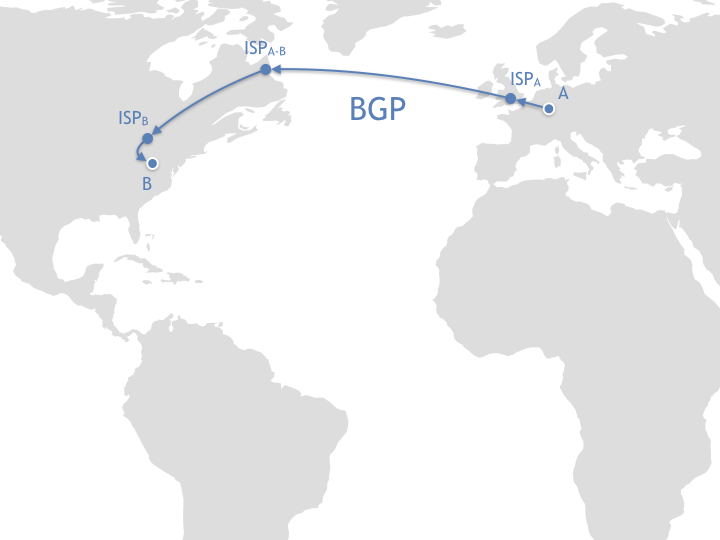
\includegraphics[width=0.97\textwidth,clip=true, trim = 0 100mm 0 0]{figures/overlay-vs-e2e002.png}
    \caption{Default data transfer}
    \label{fig:e2e-traffic}
\end{subfigure}
\begin{subfigure}{.49\textwidth}
  \centering
    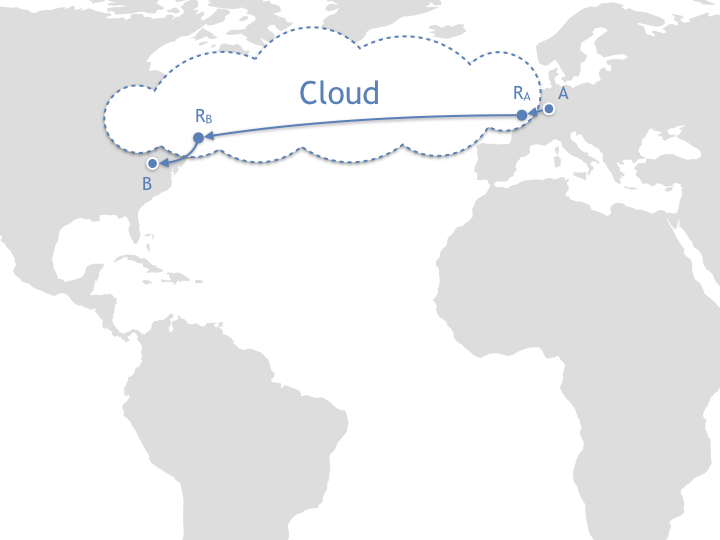
\includegraphics[width=0.97\textwidth, clip, trim = 0 100mm 0 0]{figures/overlay-vs-e2e001.png}
    \caption{Traffic through the cloud}
    \label{fig:cloud-traffic}
\end{subfigure}
\caption{Traffic from Server A in Frankfurt, Germany to Client B in New York, NY, US
}
\label{fig:e2e-vs-cloud-traffic}
\end{figure*}
%%%%%%%%%

As a first stab, consider the following simple strategy for OCD. Consider an end-host $A$ in Frankfurt that is sending traffic to an end-host $B$ in New York. We will refer to $A$ as the server and $B$ as the client. Under today's default data transport mechanisms, traffic from $A$ to $B$ will be routed along the BGP path between the two. As illustrated in Figure~\ref{fig:e2e-traffic}(a), such a path might connect $A$'s ISP to $B$'s ISP via an intermediate ISP (or more). The modulation of traffic from $A$ to $B$ in our example is determined via TCP's congestion control, which reacts to network conditions on the path (congestion, spare capacity) by adaptively adjusting the sending rate.

We consider the following simple strategy for ``cloudified'' data delivery, illustrated in Figure~\ref{fig:cloud-traffic}(b): Traffic from $A$ is sent directly to a nearby cloud ingress point and then enters the cloud. Then, traffic traverses the (single) cloud's infrastructure and leaves that cloud en route to $B$ at an egress point close to $B$. The transport-layer connection between $A$ and $B$ is split into $3$ connections, each employing TCP congestion control: between $A$ and the cloud, within the cloud, and between the cloud and $B$ (see figure). We point out that this strategy does not incorporate aspects such as employing other rate control schemes, leveraging additional relays within the cloud, traversing multiple clouds, and more. Yet, as our empirical results below demonstrate, even the simple strategy yields significant performance benefits. We will later (Section~\ref{x} and~\ref{x}) describe and evaluate more elaborate approaches to OCD.

To conclude, the simple strategy relies on:

\vspace{0.1in}\noindent{\bf Two cloud relays, one geographically-close to the server and one geographically-close to the client.} We set up, for each client-server pair, two cloud relays (VMs), selected according to their geographical proximity to the end-point (the first closest to the server and the second closest to the client). Naturally, if the server/client are already in the cloud, then the corresponding (close) cloud relay(s) is not needed. The simple strategy does not utilize any more cloud relays between the ingress and egress points, nor traverse more than a single cloud.

\vspace{0.1in}\noindent{\bf Splitting the transport-layer connection.} We break the end-to-end connection between two end-hosts into $3$ consecutive connections. As discussed in Section~\ref{x}, the challenges facing rate-control for the intra-cloud connection are fundamentally different than those faced by rate-control for the first and last connections (to/from the cloud). The simple strategy ignores this distinction and simply employs traditional TCP congestion control independently on each leg.

\subsection{Evaluation of Simple Strategy}

We next contrast the simple strategy with recent proposals for end-to-end congestion control (namely PCC~\cite{PCC} and BBR~\cite{BBR}) and also with the strategy that employs the same cloud relays but does not split the transport-layer connection, which reflects a choice to minimize the impact of BGP routing (by routing mostly within the cloud) without tampering with TCP. Our results show that the simple strategy significantly outperforms both of the other two strategies, suggesting that replacing the default congestion control alone, or the default routing alone, are insufficient. We revisit the rate-control and routing challenges in Sections~\ref{x} and~\ref{sec:numb_of_relays}, respectively.


\vspace{0.1in}\noindent{\bf Experimental framework.} 
% \hfill \break
In this section we provide results from experiments performed on three different routes; (1)~US East coast to Europe, (2)~US West coast to Mumbai, India, and (3)~US West coast to East coast. 

We used PlanetLab\cite{PlanetLab} machines as clients. 
For servers outside the cloud, we used the following:
(1)~www.cc.iitb.ac.in, located in IIT Bombay, India; (2)~www.college.columbia.edu, located in Columbia University, NY, US;
(3)~Virtual machines on Kamatera~\cite{kamatera} infrastructure, located in NY, US, and Amsterdam, The Netherlands. 
We chose university-based servers as these typically have fairly good Internet connection but do not use CDNs, and so download times are not expected to be affected by redirections or caching. We downloaded two types of files from these servers: large files (3.9~MB for the first server, 3.8~MB for the second, 10~MB for the third type), and small files (17~KB for the first server, 18~KB for the second, 10~KB for the third type). In addition, we used experimented with extra large files (100~MB) on the Kamatera servers
To assess cloud performance, we deployed relays (virtual machines) on three major clouds: \textit{AWS} (Amazon web services), \textit{GCP} (Google cloud platform) and Microsoft \textit{Azure}. In each cloud, we deployed at least one relay in each publicly-available region (\autoref{tab:cloud-config}), 
\begin{table} {\small
    \centering 
    \begin{tabular}{c c c c}
        %\hline
         Cloud &            AWS &           Azure               & GCP \\ \hline %\hline
         \# of Regions &    14 &            26                  & 10 \\
         Machine %Type/Size 
            &     t2.micro &      Standard\_DS1\_v2   & n1-standard-1 \\
         \textcent/hour &   1.2 -- 2         & 7                 & 4.75 -- 6.74 \\
         \textcent/GB & 9  & 8.7 -- 18.1   & 12 -- 23 (1 in US) \\ \hline
       
        % \hline
    \end{tabular}
    \caption{Number of regions and machine types used in each cloud, and their pricing, taken from the cloud providers' website. 
    %\IK{I deleted lines to make it look nicer and compressed to fit single column; feel free to revert. Also, very minor: would the transpose of this table look better? Feel free to ignore.}
    }
    \label{tab:cloud-config}
    }
\end{table}
yielding a total of 50 relays. Each relay ran either Ubuntu 17.04 or 17.10 using relatively cheap machine types.

For the testing of different congestion control algorithms, we used the Ubuntu BBR option, and an in-house PPC vs.1 implementation. More details regarding the Quick TCP approach can be found in~\ref{x}.

\begin{figure}
  \centering
  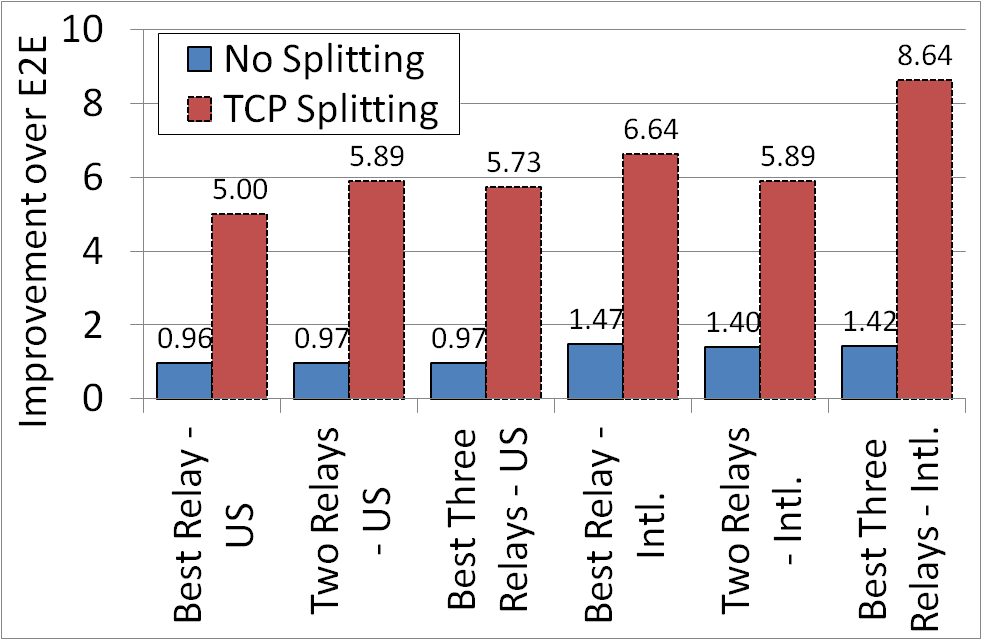
\includegraphics[width=\columnwidth,trim=2mm 2mm 2mm 2mm,clip]{figures/tcp_splitting_aws.png}
  \caption{Placeholder for straw man vs. clever e2e CC}
 \label{fig:cloud-vs-CC}
\end{figure}

\vspace{0.1in}\noindent{\bf The simple strategy \emph{vs.} clever end-to-end congestion control.} We tested the different congestion control schemas vs. cloud performance using TCP cubic using Kamatera servers (which allows us to change the congestion control algorithm). Figure~\ref{fig:cloud-vs-CC} shows the difference in performance. 
In the continental US scenario, we can see that using the cloud provides x5 improvement over Quick-Start TCP \NR{aggressive?}, and x7 over BBR and PPC.
The results for the US to Europe route differ per cloud: the best performing cloud, the improvement over BBR and Quick-Start was a staggering x20, x33 for PCC for the large file. For the extra large files, the improvement was even better, at x27.

\vspace{0.1in}\noindent{\bf The simple strategy \emph{vs.} no connection splitting.} Several papers (\ref{x,y,z}) demonstrated the need for splitting the connection, though on on a smaller scale. Our results are shown in Figure~\ref{fig:must-split}. \NR{We might want to change that one, as we're only discussing two relays at this point. We do have the data so manipulating this one shouldn't be a problem}


% To split the TCP connection we used ssh to localhost on each relay and utilized ssh's port forwarding option to forward the byte stream to the next machine en route to the destination.

\MS{Compare to BGP+TCP and to BGP+BBR/PCCv1 \\
... and to BGP+aggressive TCP? and to split not in the cloud?}




%%%%%%%%%%%%%%%%%
\begin{comment}
\begin{figure}[t!]
  \subfloat[\label{fig:must-split-aws}Using AWS relays]{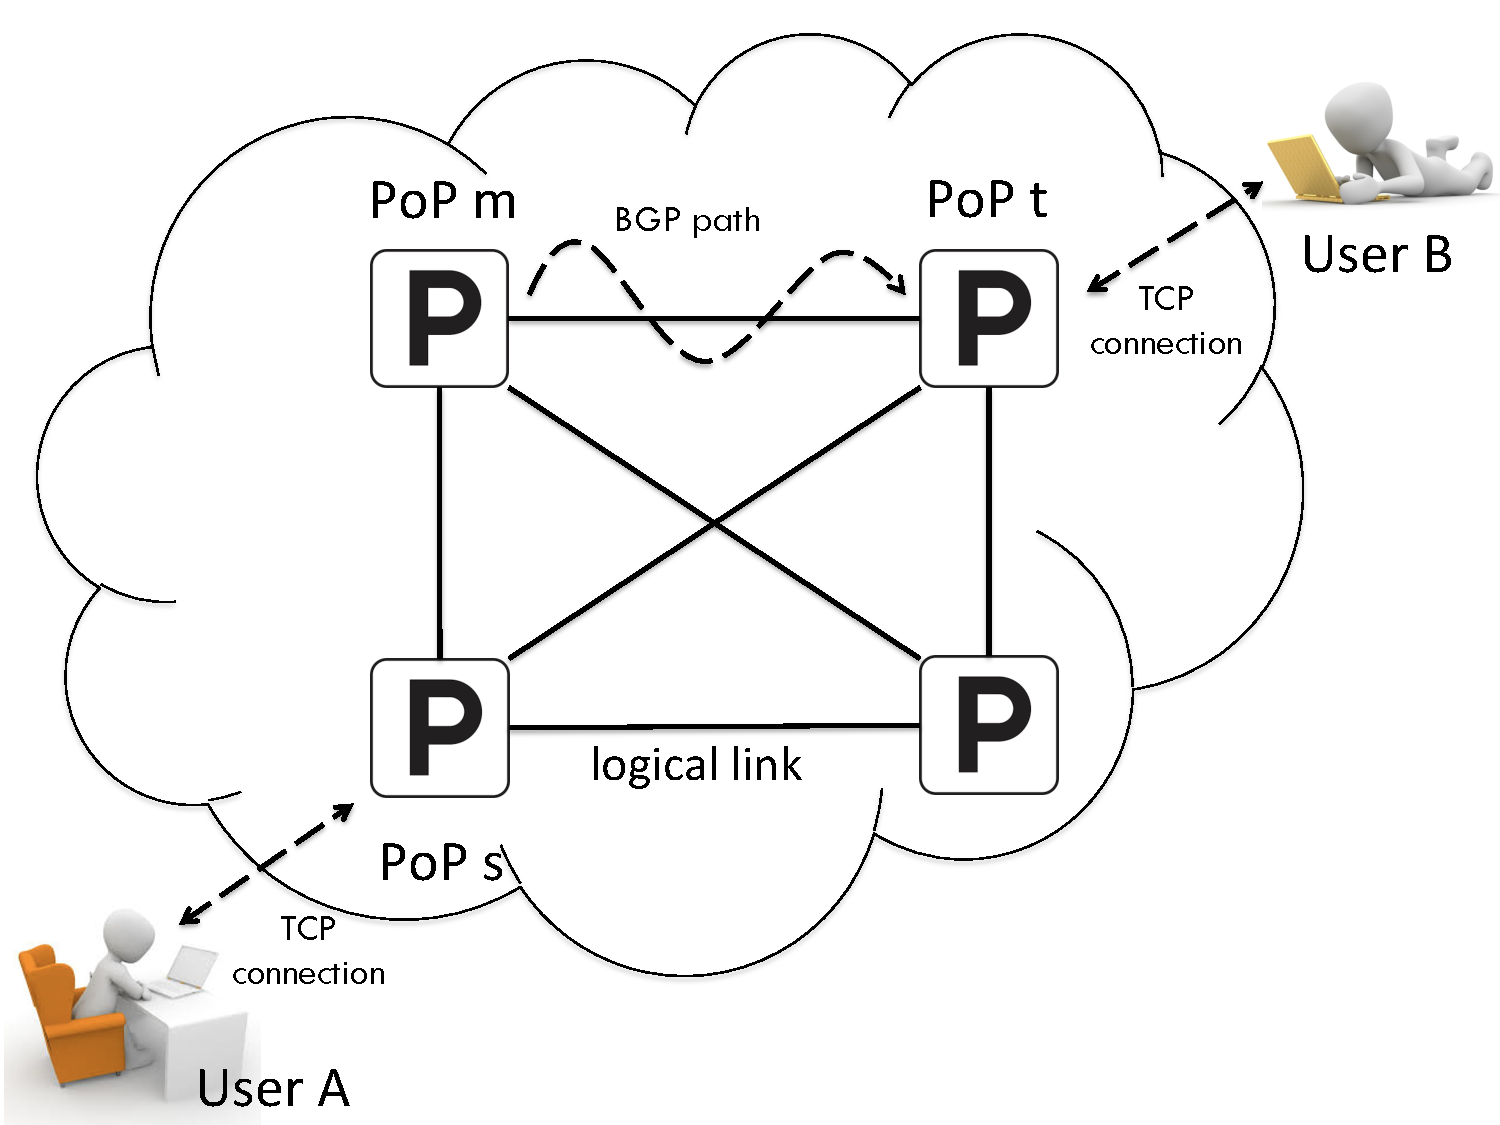
\includegraphics[width=0.2\textwidth]{overlay.pdf}}
  \subfloat[ \label{fig:must-split-aws} Using AWS relays]{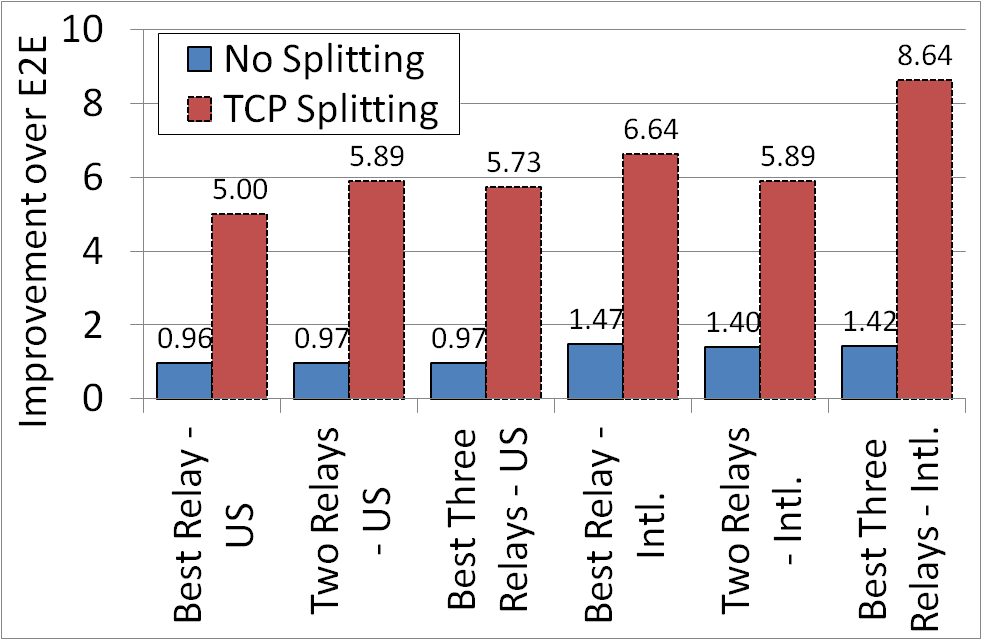
\includegraphics[width=0.2\textwidth]{figures/tcp_splitting_aws.png}}
    \subfloat[ \label{fig:must-split-aws} Using AWS relays]{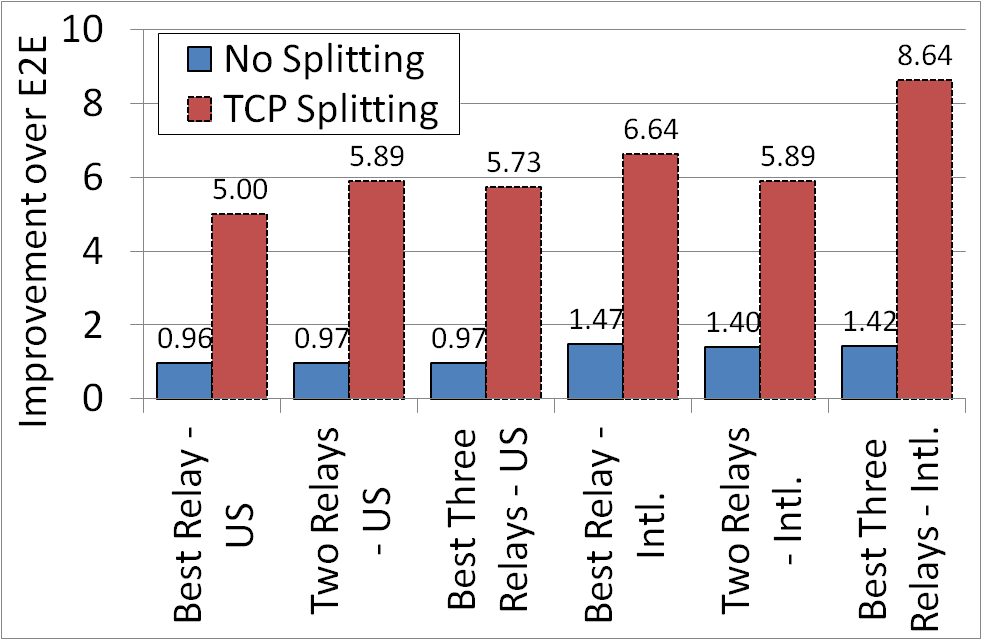
\includegraphics[width=0.2\textwidth]{figures/tcp_splitting_aws.png}}
\caption{\label{fig:tau} test}
\end{figure}
\end{comment}
%%%%%%%%%%%%%%%%%%%%%%%%%%%%%%%%%%

\begin{figure*}[t!]
  \centering
  \begin{subfigure}{.32\textwidth}
  \centering
    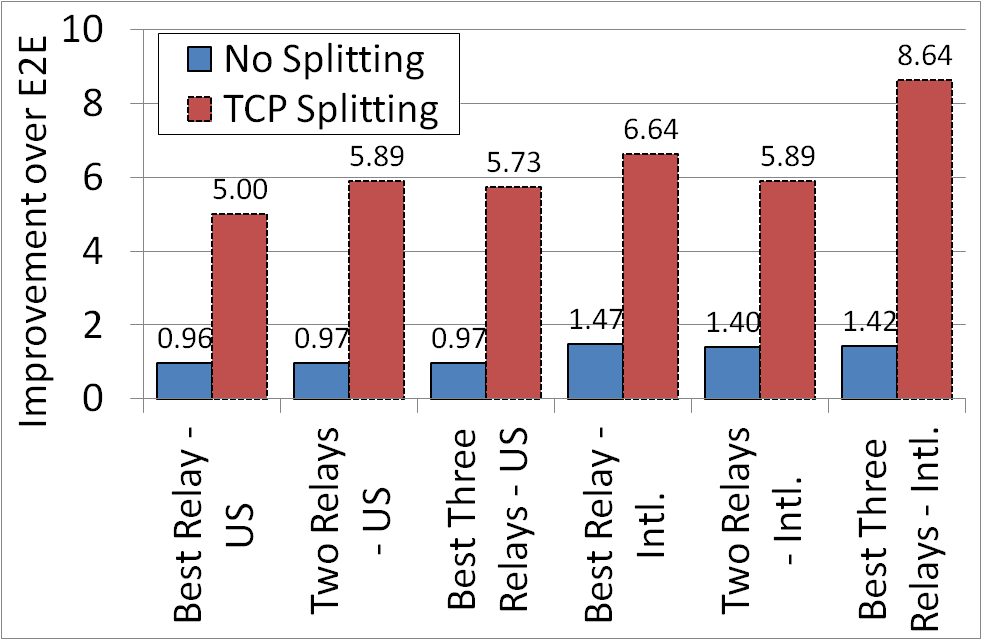
\includegraphics[width=0.97\textwidth,trim=2mm 2mm 2mm 2mm,clip]{figures/tcp_splitting_aws.png}
    \caption{Using AWS relays}
    \label{fig:must-split-aws}
\end{subfigure}
\begin{subfigure}{.32\textwidth}
  \centering
    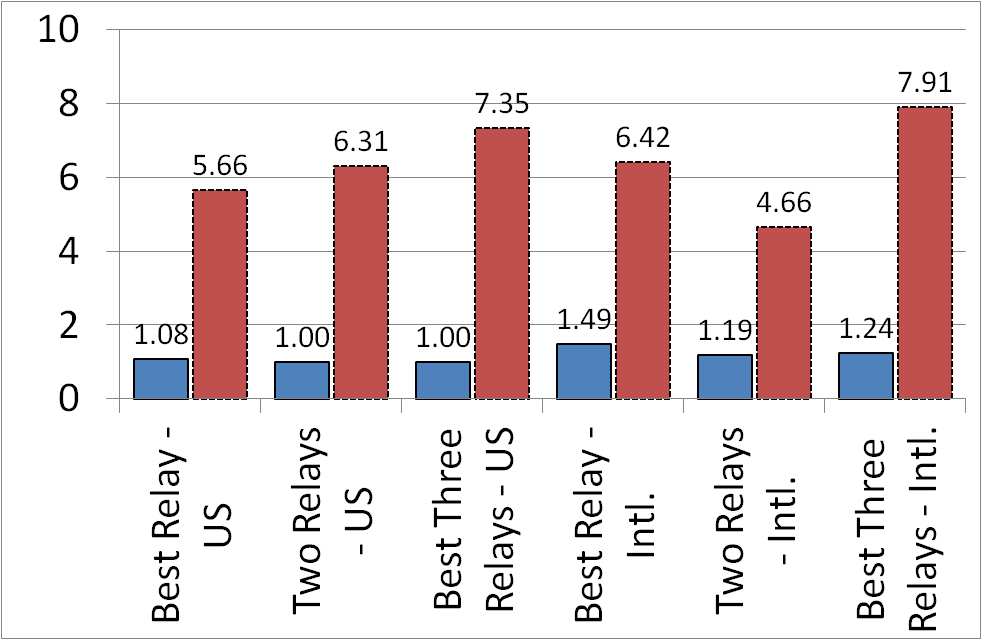
\includegraphics[width=0.97\textwidth,trim=2mm 2mm 2mm 2mm,clip]{figures/tcp_splitting_az.png}
    \caption{Using Azure relays}
    \label{fig:must-split-az}
\end{subfigure}
\begin{subfigure}{.32\textwidth}
  \centering
    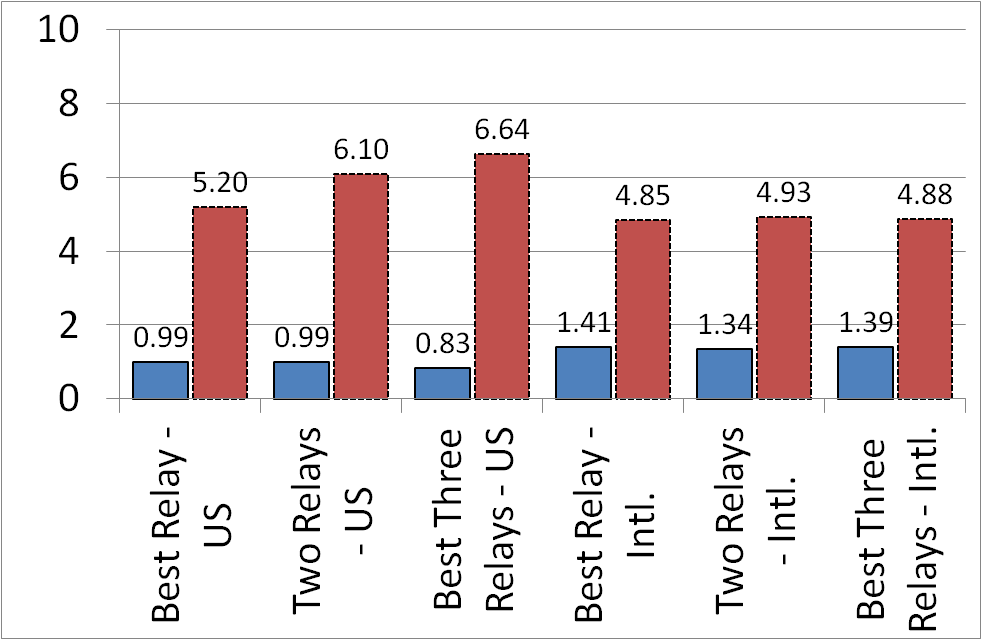
\includegraphics[width=0.97\textwidth,trim=2mm 2mm 2mm 2mm,clip]{figures/tcp_splitting_gcp.png}
    \caption{Using GCP relays}
    \label{fig:must-split-gcp}
\end{subfigure}
\caption{Evaluation of the benefits of (1) \textit{going through the cloud}; and (2) \textit{using TCP splitting}. \textbf{(1)} The left blue bars display the performance of \textit{going through the cloud without TCP splitting}. In the intra-US case, when sending a large file from New York to San Francisco, there is little performance change. For example, the best case is a 1.08$\times$ improvement with the best single relay in Azure, while the worst is the 0.83$\times$ performance in the three-relay GCP case. The international case between Mumbai and SF does display some improvement of about 40\%. \textbf{(2)} The right red bars display the performance of \textit{going through the cloud with TCP splitting}. The performance improvement is noticeably larger across all clouds. The best-single-relay and the simple-dual-relay experiments display some 5$\times$ improvement; the best-triple-relay experiments typically improve this further to some 6-8$\times$ improvements.
}
%TCP splitting is a must
\label{fig:must-split}
\end{figure*}







\section{Rate-Control Strategy}

\subsection{Our pipe dream -- ideal}

Show Split vs. Pipe and explain the challenges in the difference


\begin{figure*}[t]
  \centering
    \begin{subfigure}{0.65\columnwidth}
  \centering
  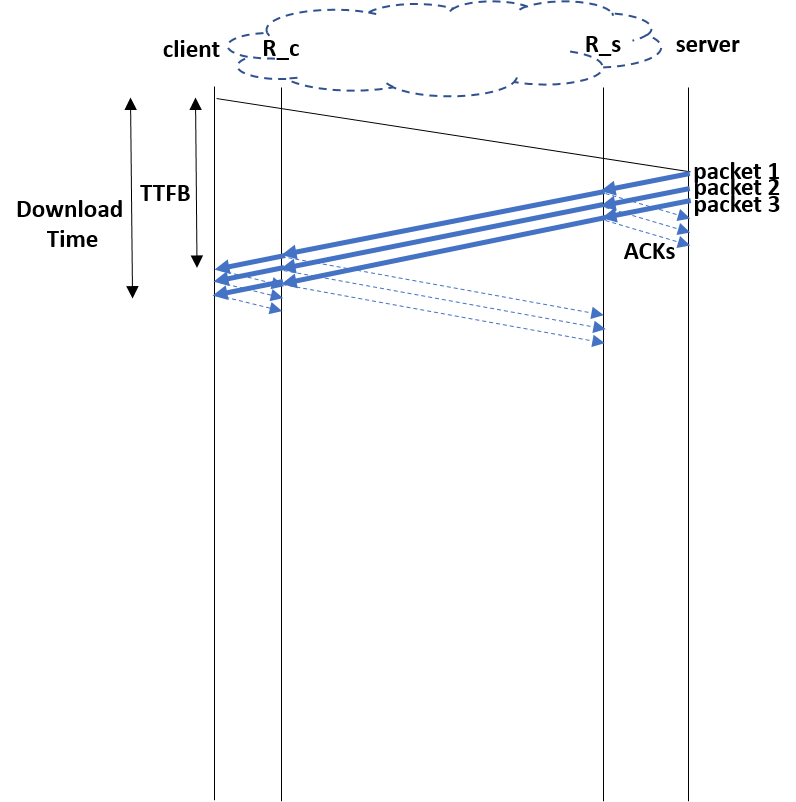
\includegraphics[width=\columnwidth]{figures/ideal.png}
    \caption{Ideal transmission.}
    \label{fig:ideal}
\end{subfigure}    \centering
\begin{subfigure}{0.65\columnwidth}
  \centering
  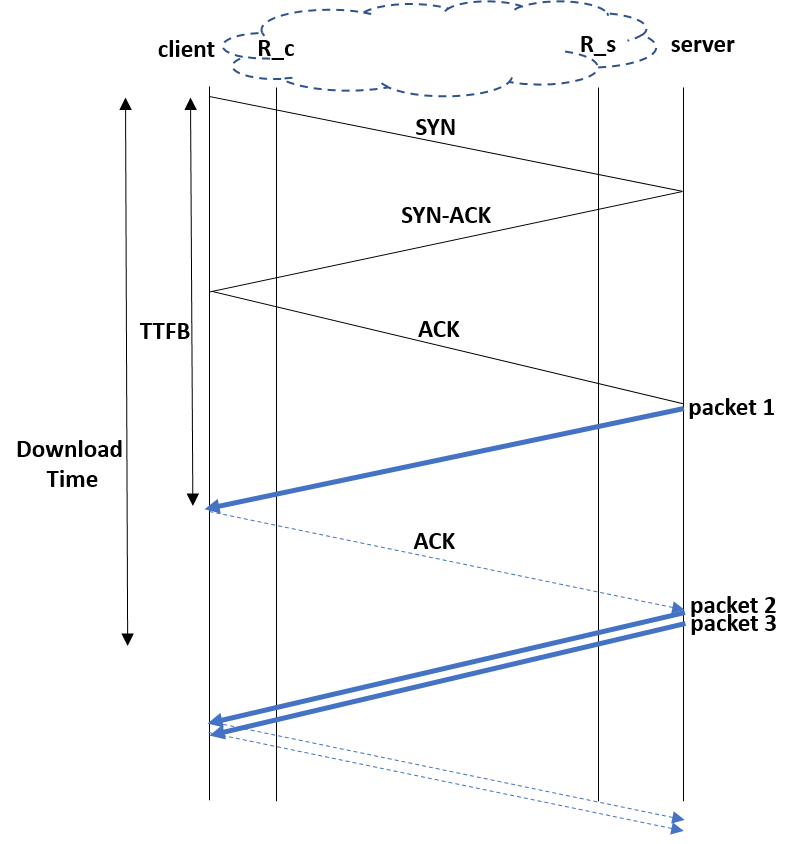
\includegraphics[width=\columnwidth]{figures/e2e.png}
    \caption{End-to-end / cloud NAT.} \label{fig:e2e}
\end{subfigure}    \centering
\begin{subfigure}{0.65\columnwidth}
  \centering
  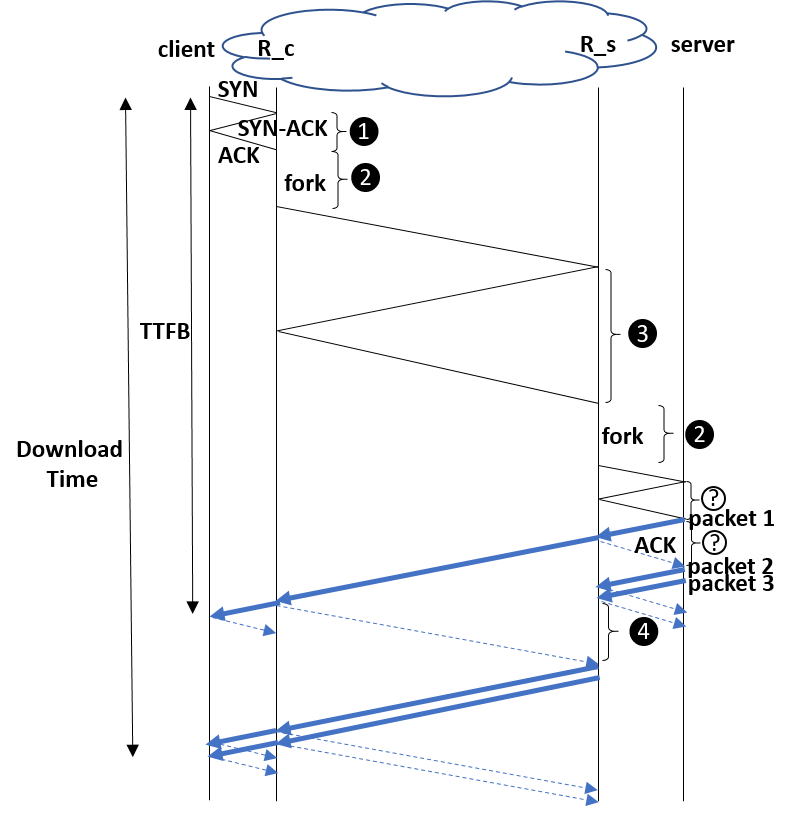
\includegraphics[width=\columnwidth]{figures/split.png}
    \caption{Simple cloud split.} \label{fig:split}
\end{subfigure}
%  \centering
% \begin{subfigure}{0.6\columnwidth}
%   \centering
%   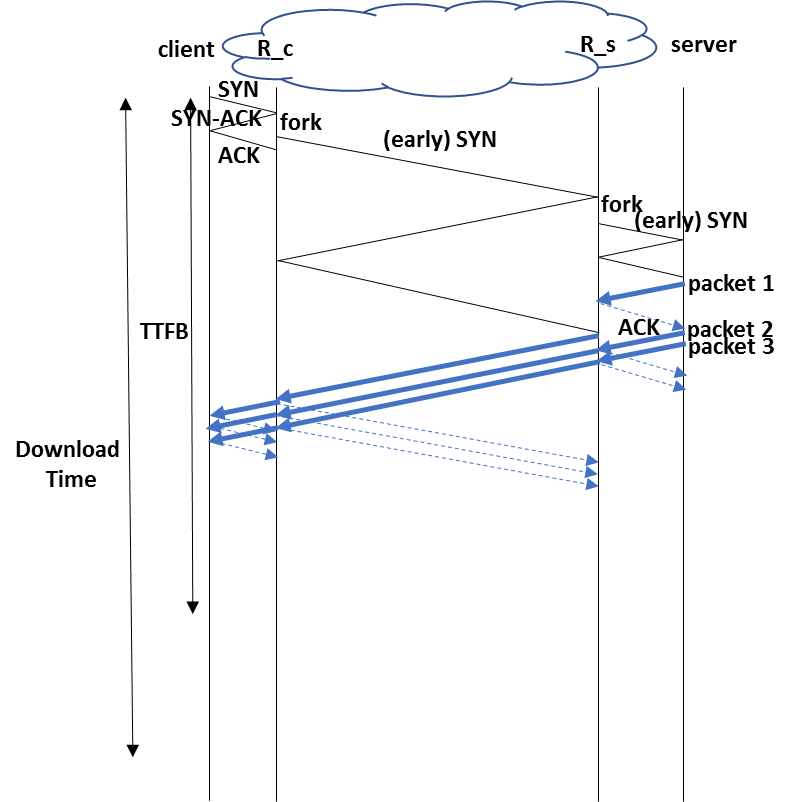
\includegraphics[width=\columnwidth]{figures/early-syn.png}
%     \caption{Early-SYN.} \label{fig:early-syn}
% \end{subfigure}
    \caption{Comparison of the baseline data transmission methods considered in this paper. For representation simplicity, we assume that the client requests three packets, that the initial TCP window size is one packet, and that there are no losses.\\ \textit{(a)} In an ideal and optimal data-transmission world, the request for packets goes through directly, and the packets are then sent in a pipeline-like fashion to the client. Therefore, the time-to-first-byte (TTFB) is just one round-trip time (RTT), which is as low as it can get. The download time is barely higher.\\ \textit{(b)} Today, an end-to-end TCP transmission first requires the establishment of an end-to-end connection, which adds one RTT to the ideal time. (The case of a transparent cloud NAT is essentially the same and represented in the same figure. The routers are then in the cloud and the RTT can be slightly different.) In addition, waiting one RTT for the first ACK further delays the download. \\ \textit{(c)} Finally, to decrease the download time and get closer to the optimum, we start with a standard TCP split in the cloud. We find that while  we can decrease the ACK time, we also get new delays and especially the thread forks. \\
    Our goal is to obtain an implementation that gets closer and closer to the ideal time. We find that using \textit{Early-SYN}, we can remove the SYN-ACK and ACK delays marked as (1) from the critical path. Next, using a \textit{thread pool}, we can remove the forks (2). Then, with a \textit{connection pool}, we can eliminate delay (3). Finally, we present an aggressive TCP that prevents delay (4). There are only two last delays that we did not remove on the road to optimality (marked as ?): the last connection SYN-ACK/ACK, and the first data ACK. Both depend on the server parameters, and we assume that we cannot change these. (But if we can, we are essentially at the optimal point!)      \IK{TBD} }
\end{figure*}

%\subsection{} \IK{See below -- When Alex is done editing the file, it corresponds to the following section which needs to become a subsection}

%Clever splitting (recycling connections etc.)

\subsection{KTCP Design} \label{sec:design}
\subsubsection{Design Goals}
The aim of KTCP split is to provide uncompromising TCP optimization, while, utilizing commodity VMs. Easily deploy-able commodity VMs in a public cloud environment, provide a powerful and flexible platform for our goals. We implement KTCP as a kernel module for Ubuntu 16.04. We use the ubiquitous POSIX socket API as the basis for our TCP proxy.  
Implementing KTCP in the kernel allows us; to take advantage of resources only available in the kernel and avoid the penalties that stem from numerous system calls ~\cite{Copy, FlexSC}. We add several proc ~\cite{proc} files to control the behaviour of KTCP. 

\T{Basic implementation} The basic design of our TCP proxy, shares a common form with other open source implementations ~\cite{SOCKS, WhatEverAranIsUsing}. The design has three basic steps. We create a socket that listens for incoming connections. Iptable ~\cite{iptables} rules redirect TCP packets to our proxy socket. A second TCP socket is used to connect to the destination. All bytes of the stream are read from one socket and then forwarded to its peer.

\T{Early Syn} In early syn ~\cite{Ladiwala}, a syn packet is sent to the next-hop server as soon as the syn packet arrives. This without waiting for the three way handshake to finish. Standard POSIX socket API doesn't facilitate the capture of the first TCP SYN packet. We utilize Linux netfilter~\cite{netfilter} hooks to captures this first SYN packet and trigger the start of a new connection. This allows the proxy to establish the two connection in parallel. 

\T{Thread Pool} Each new proxy connection is handled within two dedicated kernel\_threads. Each thread receives from one socket and writes to its peer. Unfortunately, the creation of a new kernel\_thread is costly on our setup it takes XXX milliseconds\MA{I plan to run a small experiment to measure the time it takes to create a kernel\_thread, a fork and a POSIX pthread}. This delay is added to the time to first to byte. To mitigate this problem, we create a pool of reusable kernel threads. We create a list of pre-allocated kernel\_threads. Each kernel\_thread is initially in TASK\_INTERRUPTIBLE state; when the thread is allocated the task is scheduled to run and a function to run is set , when the function is completed the thread return to state TASK\_INTERRUPTIBLE; awaiting for a new function to run \MA{awkward needs a rewrite}.A pool of pre-allocated kernel threads thus removes the overhead of new kernel\_thread creation, as a new connection initialization can start immediately.

\T{Reusable connections} Another optimization we implement, aims to eliminate the delay of the three way handshake between two proxies. We create a pool of connections between two distant proxies. The sockets are configured with KEEP\_ALIVE. On early syn we allocate a connected socket from our pool and use it for the connection; thus eliminating the three way handshake time. Before we start forwarding the data we send the destination address on the connection it self, all following bytes belong to the original stream. 
This element has a server and a client part. The server has a dedicated socket that accepts connections from peer-proxies. These connections wait for for the destination address, when the destination address is received a connection is established and the bytes are forwarded between the sockets just like in the basic design. Nagel's Algorithm ~\cite{nagel} should be disabled on these sockets; sockets configured TCP\_NODELAY. In our experiments we have seen that; without this configuration, time to first is increased by 200 milliseconds.  

\T{Design Considerations} While most optimizations we propose in KTCP, can be implemented in user space, and thus provide an easier development environment. Netfilter ~\cite{netfilter} is the natural option for capturing the syn packet and this option is only available via a kernel module. Additionally, numerous system calls can hinder performance considerably ~\cite{Copy, FlexSC}\MA{An experiment that shows this could be beneficial}. By working in the kernel, we eliminate the redundant transitions to and from user space. The decision to implement KTCP in the kernel is farther made easy, by the fact that, all socket API have a kernel counterpart. One problem with an in kernel implementation is that epoll ~\cite{epoll} has no kernel API. We believe that context switching between kernel\_threads may become an issue with scale. We evaluate the context switch time and find that it takes YYY Yseconds \MA{Need to run this test}.

\T{Proc} The size of the thread-pool, the destination of a pre-connection and the number of pre-connections are controlled via the proc fs~\cite{proc} interface.

\T{Extreme performance} \MA{This paragraph is just my ramblings on performance, this whole discussion is gratuitous}For a very large number of connections it may become necessary to expand the epoll API to the kernel. Socket API in the kernel is not zero copy, expanding the socket API is possible but not trivial, copying data can become an issue with scale ~\cite{Copy}. Network I/O is serviced with interrupts, on virtual machines this usually means costly VM exits ~\cite{Eli, Elvis}. Additionally it is well documented that para-virtual devices like ~\cite{virtio,vmxnet3} have a penalty to performance ~\cite{Eli, Elvis}. An SRIOV device and a machine with a CPU that supports Intels vt-d posted interrupts may be needed to achieve near bear metal performance.


\subsection{Rate-Control Within the Cloud}
Aggressive TCP

\subsection{Congestion Control at the Edge}

TCP/BBR/PCC at the edge -- need to check: for Noga: what's the story here? \NR{Technically the e2e results are the same experiments, unless we'll use the client in SF. Changing only in the Server doesn't do much at all, especially for the file size we're currently using. There could be a change for 100K / 1M files (that's what Aran saw when changing the CC for cloud machines in the last iterations), but I'm not sure it's that interesting to add}

\subsection{Putting it all together: We are close to Pipe}

\subsection{Experiments: improving the strawman}

\section{Routing Strategy}

\IK{Do we want to include the results here, or only mention strategies then have an experimental section?}

1 vs. 2 vs. 3 relays, intra-cloud vs. multiple clouds, ...


\IK{Also need to check going through points outside the cloud: here are settings we mentioned:\\
1. France-Switzerland-Prashanth(SF)-Israel(SF), or\\
2. France-Switzerland-Amazon(SF)-Israel(SF), \ie half cloud}


\subsection{How Many Relays?} \label{sec:numb_of_relays}
%\IK{feel free to have another title here}
%How Many Relays?} \IK{Or: ``What Relays?"}
%When using an overlay network, one may ask, how many relays are too many?
%We began by trying all the options for a single relay. In addition, we tested the simple heuristics of using the relays, one closest to the client, and the other closest the the server. Finally, we  tested adding the nodes that performed best as single relays to the formally mentioned two relays. \NR{Per IK's changes to the Methodology, do we want to remove this paragraph?}



%Let's focus on the cloud relay options of \autoref{fig:must-split}. It is not clear that we have to either pay for two relays, 

\begin{figure}
  \centering
    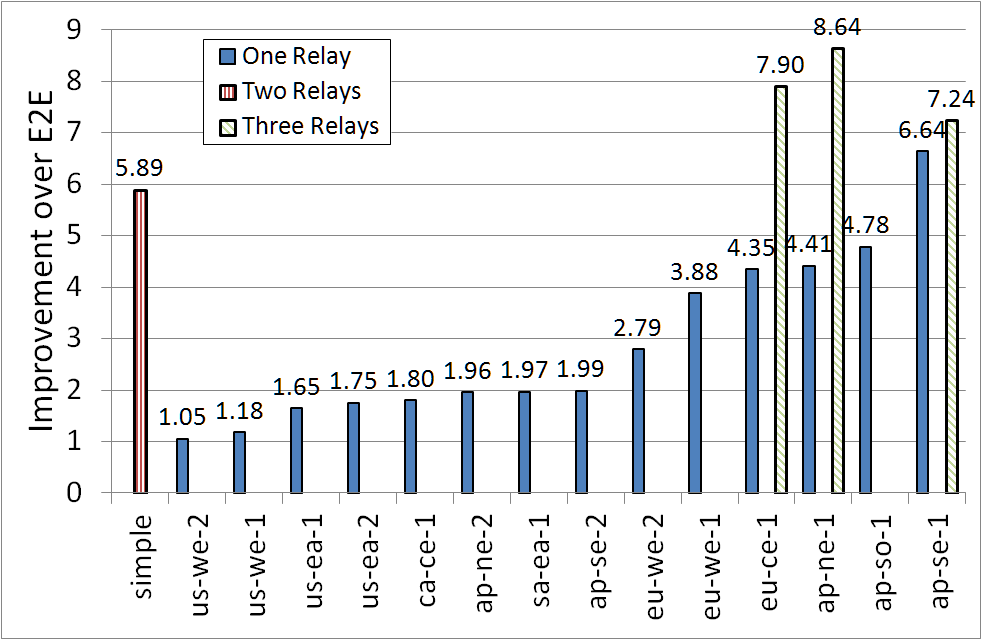
\includegraphics[width=\columnwidth,trim=2mm 2mm 2mm 2mm,clip]{figures/hops.png}
    \caption{One, two and three relays when using  TCP splitting in AWS for the Mumbai-SF international setting. (1)~The first striped red bar shows the performance of the simple unoptimized two-relay placement at the nodes that are closest to the client and the server. (2)~Next, the 14 blue bars show all the options for a single-relay option. The best option is ap-se-1 with a normalized performance of 6.64$\times$, above the two-relay option. However, all other single-relay options have a lower performance, and the    median option gets 1.99$\times$, \ie only 30\% of the best performance. (3)~Finally, the three green bars show a few options for the middle relay in the three-relay method, given the simple two-relay options at the extremities; \eg eu-ce-1 shows the performance of consecutively going through (us-we-1$\to$eu-ce-1$\to$ap-so-1). The best option is ap-ne-1 with an 8.64$\times$ performance.} 
    \label{fig:how-many-hops-aws}
\end{figure}

Our straw man proposal in section~\ref{sec:straw_man} uses two relays, where the first is the one which is geographically the closest to client, and the second to the server. To choose this methodology, we ran extensive experiments through multiple scenarios.

% How hard is it to identify the best \emph{single} relay? \autoref{fig:how-many-hops-aws}
%After considering Figure~\ref{fig:must-split}, one might be inclined to think that a single relay might provide better performance than the two relays, chosen by using our simple approach. 
Figure~\ref{fig:how-many-hops-aws} extends \autoref{fig:must-split-aws}, showing the results for all the relay options tested in AWS using TCP splitting in the international case. 
We learn that (1) all but one relay perform \emph{worse} than the simple two-relay option; (2) the \emph{best} single relay (ap-se-1, \ie ap-southeast-1 in Singapore) indeed performs better than our simple two-relay approach, but this relay is neither the closest to the client, nor the closest to the server, nor the (geographically) closest to the mid-point. 

This suggests that determining the identity of the best single relay to use is nontrivial as this relay seems to have no obvious characteristics. While \autoref{fig:how-many-hops-aws} shows results for relays in AWS, similar results were observed when using GCP and Azure.


\subsection{Mixing Clouds}

We also tested whether routes traversing different clouds can produce better results. To this end we rerun the 2-relay and 3-relay experiments (with TCP splitting) using the SF client and Mumbai server with \rc on AWS and \rs on Azure. We compared performance to that of the same strategies with AWS relays only. Our preliminary results show that mixing clouds was indeed beneficial in some of the evaluated scenarios--- specifically, when Quick-Start Cubic was used and/or when three relays were used (with either Cubic or Quick-Start Cubic). 


%%%%%%%%%%%%%%%%%%%%
\section{Deployment Strategies}

We next discuss strategies for deploying OCD. We consider two different contexts: (1) a cloud provider deciding to provide OCD as a service, and (2) another entity (say, a website) deciding to employ OCD for its traffic.

\subsection{Enhancing Cloud Services with OCD}

Similarly to the transition to cloud computing, cloud service providers such as Google, Amazon, and Microsoft, can leverage their resources (VMs, network capacity) to broaden their business offerings to customers by providing transit services to others.

Realizing OCD by a cloud provider can be accomplished by utilizing mechanisms employed by CDNs~\cite{x,y,z}, such as the following. Suppose that a content owner, say, CNN, wishes traffic to/from the content to be sent via OCD and purchases OCD services from the cloud. The cloud service provider can then set up cloud relays in the vicinity of the CNN content (and autoscale them as needed). Now, consider a client $A$ located outside the cloud. When the client seeks CNN's IP address through DNS, the corresponding DNS records should be overridden so as to point that client to the IP address of the cloud relay closest to that client. Then, traffic from the client to CNN and vice versa can be sent through the cloud by entering/leaving the cloud via the corresponding cloud relays.

\subsection{Incremental Deployment of OCD}

Consider now the scenario that a content owner such as CNN wishes to transition to OCD yet no cloud service provider offers OCD as a service. CNN, in this example, can deploy OCD for its own traffic using the exact same methodology as in the Section~\ref{x}. Of course, the overhead of doing so is non-negligible (overriding DNS records, setting up virtual machines in the cloud and autoscaling them, etc.). Alternatively, non-cloud-service-providers can offer such services to content owners (such as CNN) by creating a virtual overlay over the cloud and contending with the associated operational challenges.

Regardless of how this is accomplished, \emph{incremental} transition to OCD over a cloud infrastructure, i.e., the scenario that some traffic traversing the cloud is modulated as discussed in Section~\ref{x}, and other traffic is not, raises questions about how friendly OCD traffic is to other flows on the cloud infrastructure... Results!


\section{More Experimental Results}

\IK{Important: can we tell them that they can play with something online? If not, can we promise them that there is some open-source code? Or even some VMs that they can download and run? Being able to replicate the results is important in this community, and the clouds help us  enable cool stuff.}
\AB{I think we can publish the scripts we currently use (or a modified version of these scripts...) and add a README on how to run them. No need for a special VM. Just need to create VMs in the clouds (and we can also publish scripts for that).}

% In preparation for this paper, we ran of thousands of experiments \AB{actually - > 240K downloads by me and > 140K downloads by Noga. I don't know if I would call each an "experiment", though}, considering both inter-continental and intra-continental routing. For the sake of simplicity, we focus in this paper on representative examples, before discussing a few trends and outliers.
% . While not exhaustive by any means, they included various routing options: for example, West US to Mumbai via Asia, East US to Mumbai via Europe, and regional routing in Asia, Europe and the Americas. In the following chapters we discuss some of the trends observed, as well as outliers. 


% \noindent{\bf Clouds.} We deployed relays (virtual machines) on three major clouds: \textit{AWS} (Amazon web services), \textit{GCP} (Google cloud platform) and Microsoft \textit{Azure}. In each cloud, we deployed one relay in each publicly-available region (\autoref{tab:cloud-config}), 
% \begin{table}[t] {\small
%     \centering 
%     \begin{tabular}{c c c c}
%         %\hline
%          Cloud &            AWS &           Azure               & GCP \\ \hline %\hline
%          \# of Regions &    14 &            26                  & 10 \\
%          Machine %Type/Size 
%             &     t2.micro &      Standard\_DS1\_v2   & n1-standard-1 \\
%          \textcent/hour &   1.2 -- 2         & 7                 & 4.75 -- 6.74 \\
%          \textcent/GB & 9  & 8.7 -- 18.1   & 12 -- 23 (1 in US) \\ \hline
       
%         % \hline
%     \end{tabular}
%     \caption{Number of regions and machine types used in each cloud, and their pricing, taken from the cloud providers' website. 
%     %\IK{I deleted lines to make it look nicer and compressed to fit single column; feel free to revert. Also, very minor: would the transpose of this table look better? Feel free to ignore.}
%     }
%     \label{tab:cloud-config}
%     }
% \end{table}
% yielding a total of 50 relays. Each relay ran Ubuntu 17.04 using relatively cheap machine types. \NR{We actually deployed more than one machine. Also, we used Ubuntu 17.10 for the PCC machines.}
% \IK{simple machines}
%\AB{For the US experiments we used fewer regions -- we only used the regions the Americas. We should put that somewhere.}
%\NR{We actually deployed more than one VM per region, Aran has the total, but I'm guessing we had 100+ machines}
%\NR{@AB, you have the setup of all of the machines you deployed for both you and me, right?}\AB{For the Mumbai experiments I used all regions of the cloud provider tested. I.e., all 10 from GCP, 14 from AWS and 26 from Azure. For the US experiments I used the regions in America (i.e., all US regions and Canada and South America, if they exist for the particular cloud provider)}\NR{So, how do we want to fill this out?}
% \begin{romanlist}
%     \item AWS - 14 regions
%     \item GCP - 10 regions
%     \item Azure - 26 regions
% \end{romanlist}\AB{did we define these acronyms?}\NR{Nope, maybe it's a good place to do so}
% . 
%, and was used as either clients, relays, or servers\AB{So, will we have graphs were the VMs are used as servers? Do we want to call the VMs relays, Relays, Jump-hosts? Something else? (just to be consistent)}. \AB{I think that for this paper we should concentrate on clients and servers on the Internet (not the cloud), or at least - on a server on the Internet...}

% \smallskip\noindent{\bf Servers.} We used several university-based servers: 
% %For servers outside of the cloud, we have used to following: 
% (1)~www.cc.iitb.ac.in, located in IIT Bombay, India; (2)~www.college.columbia.edu, located in Columbia University, NY, US;
% \NR{Should note that these are no longer available}
% (3)~www.biomed.drexel.edu, located in Drexel University, Philadelphia, PA, US;
% (4)~www.uni-frankfurt.de, located in Goethe-Universität Frankfurt am Main, Frankfurt, Germany
% %The files from the first server were reused in the cloud servers. 
% We chose university-based servers as these typically have fairly good Internet connection but do not use CDNs, and so download times are not expected to be affected by redirections or caching. We downloaded two types of files from these servers: large files (3.9~MB for the first server, 3.8~MB for the second, 8.9~MB for the third, 9~MB for the fourth), and small files (17~KB for the first server, 18~KB for the second, 9~KB for the third, 24~KB for the fourth).
% %Our bandwidth tests relied on the large files. \AB{Do we need the last line?}
% % \NR{Should I just create a table?}

% % \smallskip\noindent{\bf Clients.} We used three types of clients: (1)~ a personal computer located in San Francisco (SF), connected to the Internet through Comcast; (2)~PlanetLab~\cite{PlanetLab} nodes in multiple locations worldwide; and (3)~Kematera~\cite{x}
% % ; and
% %   \item % and running Ubuntu 16.04.2 LTS (Linux kernel verion 4.8.0-52).
% % \end{romanlist}

% \smallskip\noindent{\bf Data delivery strategies.} For each \textit{(client, server, cloud provider)} triplet, we downloaded small and large files, employing the following data delivery strategies:

% %\begin{CompactEnumerate}
%  % \item 
% \PST{End-to-End (E2E).} Download via the default, BGP-based Internet route between the client and server. This is the baseline against which all other strategies are compared;
% %   \item \label{item:nat-1hop}

% \PST{One relay.} Traffic is routed through a single relay node in the cloud. We run this experiment for each and every one of our deployed relays in the specific cloud (except for intra-US experiments, where we only use relays in the American continent).
% % \IK{can we say from the start that we always use the same node in each region, and write here ``the" node for simplicity? it will help the writing everywhere} \NR{Aran and I used different machines, and also these might}

% %\AB{I dropped the Availability Zone discussion. We are short on space as it is.}
% %We use only a single availability zone in each region. \IK{elaborate on the last line: do we know if it matters?} \NR{I'm not sure what it means} \AB{Each region has 2 or 3 availability zones - each connected to a different power supply, possibly situated in a different physical location and might be connected to the network/Internet through different links and different ISP/IXP. A more rigorous test would need to create a node in each availability zone. This is mentioned for completeness of the description.} Thus, a cloud with $n$ regions yields $n$ relay nodes and $n$ corresponding experiments.
% %   \item \label{item:nat-2hop}

% \PST{Two relays.} Traffic is now routed through 2 relays (in the same cloud), such that the first (denoted $\rs$) is closest to the server RTT-wise and the second ($\rc$) is closest to the client RTT-wise (going over all possible combinations of relay-pairs would be prohibitive). The two relays are always distinct in our experiments. %\IK{Aran: in addition to our discussion that you should mention geographical proximity: have a look at what Michael wrote in the intro under "A simple routing strategy fares reasonably well"}
% In retrospect, the geographically-closest region to the client (server) is almost always the one with the minimum RTT.
% %to establish our two relay nodes, we choose , where the first relay is chosen in the cloud provider's region closest to the client, and the second in the region closest to the server. ``Closest'' here means the region with the smallest RTT to client or server, respectively;
% % \item \label{item:nat-3hop} 


% \PST{Three relays.} Traffic is routed through 3 relays (in the same cloud), with the first and last relays ($\rs$ and $\rc$, respectively) chosen as described above, and, for each of the other relays, we run an experiment with that relay as the intermediate relay between $\rs$ and $\rc$. For intra-US experiments we only use intermediate relays in the Americas.
% %node the third one is taken from one of the remaining regions the cloud provider operated in (again - looping over all such remaining regions);
% % \item \label{item:split} 

% \PST{Splitting end-to-end congestion control.} Repeat all of the previous experiments, this time splitting the end-to-end congestion control connection at each relay; \eg in the 2-relay experiment, a session is established between the server and \rs, a second between \rs and \rc, and a third between \rc and the client.

% We repeat this experiment for four congestion control schemes (we only change the congestion control in the cloud nodes and do not modify the end-nodes):
% \begin{CompactEnumerate}
%       \item \textit{TCP Cubic} with default settings;
%       \item \textit{Quick-Start Cubic}: TCP Cubic with large initial cwnd, initial rwnd, and socket buffer;
%       \item \textit{BBR} \cite{BBR}; and
%       \item \textit{PCC} \cite{PCC}.
% \end{CompactEnumerate} 
% % \item \label{item:cc} 
% % For each option measured in \ref{item:split} we examine three different congestion control settings for relay nodes:
% %\end{CompactEnumerate}
% We ran all the experiments in a 4-week period, in July and August 2017, at different times of day. We repeated each of the above 50 times and computed averaged results.

% \ifblind \else
% \smallskip\noindent{\bf Tools and techniques.} \textit{RTT measurements} are conducted using hping3 \cite{hping3}, by sending 20 SYN packets (at 0.1 seconds intervals) to an open TCP port on the other side and measuring the round-trip-time between sending each SYN and getting its corresponding SYN-ACK. The minimum of these 20 measurements is taken as the RTT between the two tested endpoints. We chose this method over ping so as to avoid the risk of ICMP filtering.

% \PST{Routing through relays.} Routing through cloud relays without splitting the connection was performed by using NAT on the cloud machines, configured using Linux's iptables \cite{iptables}. NAT is used so that the return path traverses the same relays.

% \PST{Splitting the connection.} To split the TCP connection we used ssh to localhost on each relay and utilized ssh's port forwarding option to forward the byte stream to the next machine en route to the destination.
% \fi


% %\IK{We didn't mention when we ran the experiments, and for how long; or that the standard deviation was sufficiently small that 50 are enough...}
% %\AB{added a short paragraph. Does not yet address the STDEV...}

% % % These different methods form a set of measurements which were repeated over 50 iterations (or more). We repeated this experiment for the three different cloud providers we considered.
% % \AB{Do we need to describe exactly how we set up the routing with and without splitting through the relays?}

% %\IK{\emph{Big decision we need to talk about:} should we organize the paper by topic, or adopt an evaluation-oriented order by first showing a run from SF to NY, then change the cloud, then change the client, then change the server?\\ Also we need to decide whether we prefer CDFs or bars showing averages: CDFs are more complete, bars easier to understand.}



% \IK{References to related work should probably go to the Intro; move/delete this next paragraph?}
% {\small
% Previous studies~\cite{CRONets} suggested TCP splitting\AB{Did we elaborate on what this means and how we do it somewhere above?}\NR{Nope, I think we should put it in with the methodology portion} would improve performance. Our first goal was to quantify the affect of this feature across multiple scenarios. 
% We experimented using inter-continental routes as well as regional routes, and the three different clouds at our disposal.\AB{perhaps this should be included in the methodology section?}
% For brevity, we only show the benefits of splitting when default Cubic is used as the congestion control algorithm in the relay nodes, and compare it to simply routing through the cloud nodes using one, two or three relays on the cloud.
% }

\subsection{TCP Splitting is Crucial} 

We start by evaluating the benefits of 
\begin{inlinelist}
    \item \textit{going through the cloud} through one, two, or three relays,  instead of the regular fully-Internet-based E2E (end-to-end) route; and \item \textit{TCP splitting}.
\end{inlinelist} In all cases, the average bandwidth results are normalized by the average bandwidth in the E2E experiment.

%\autoref{fig:must-split-aws}--\autoref{fig:must-split-gcp} 
\autoref{fig:must-split} shows the results for two main scenarios: an internal US connection between the SF client and the NY server, and an international connection between the SF client and the Mumbai server. %It differentiates the benefits by considering different data delivery methods in all three clouds.\AB{not sure what the last sentence means.}

The main take-home messages are that (1) going through the cloud without TCP splitting is not particularly helpful; (2) TCP splitting remarkably accelerates download; (3) the simple two-relay placement and the best single relay provide comparable improvements over E2E download; (4) using three  relays can typically (for the proper choice of relays) strictly improve over the 2-relay strategy.
 %\IK{please check if you agree with the conclusions} \NR{@Aran, we didn't check all the 4 node options, right?}\AB{If you mean 4 relays - I only have one experiment with this setup. Why do you ask?}
 
Why does TCP splitting have such a positive effect on performance? We argue that the reasons are as follows. TCP's performance in steady-state is reciprocal to the RTT between the end-points~\cite{mathis1997}. Splitting the link between the end-points results in path-segments with shorter RTTs, and therefore better performance. Also, a shorter RTT enables much faster ramp-up of the transmission rate during TCP slow-start. Our experiments show that in the long-haul section of the path, TCP is in slow-start during the entire download period (\S\ref{subsec:quick-start}). Yet another reason is TCP's innate unfairness towards long RTT flows. Whenever the TCP flow competes with other flows on some bottleneck along the path, it is suppressed by flows with lower RTTs.



% performance of various data delivery alternatives for six different scenarios, \ie 
% using the same client-server pair, and different cloud providers for relay nodes. The client is the San Francisco client, and the server is in Mumbai (utilizing an international route).
% Each bar represents the gain of this routing option over the regular E2E option. For the single-relay and three-relay options, both with and without TCP splitting, we only show the gain of the best performing region out of all the regions used for each of these options.

%\IK{should we insert philosophical comments on the costs of  1 optimized vs 2 naive; or of splitting?}

%It is clear that for each hop-count variant we used the better option is to employ TCP splitting. This is also true for the regions not presented in \autoref{fig:must-split}. Using TCP-splitting either has the same or better performance than the same routing option without splitting.

% In \autoref{fig:must-split-gcp} and \autoref{fig:must-split-az} we see the same trend for the other cloud providers we used for the relay nodes.



\subsection{TCP is Enough} 
%While the effects of congestion control in overlay networks have been discussed before(~\cite{CRONets}, \NR{are there any more?}), much is left unknown.
We tested the performance of the default TCP Cubic against the recently proposed BBR with the same international setting on AWS using TCP splitting. Note that we only deployed BBR  on the relay nodes and not at the end-points.
%The results of our experimentation across all scenarios yielded similar results. 
As shown in \autoref{fig:aggressive},
%showcases representative results. %The experiment setting is a personal computer client in the San Francisco area (SF), relays in AWS, and a web server in Mumbai. As can be seen in the figure, 
BBR did not achieve better performance than default TCP.
%BBR was activated in all the relay nodes. It did not help in achieving better performance.

% \begin{figure}
%   \centering
%     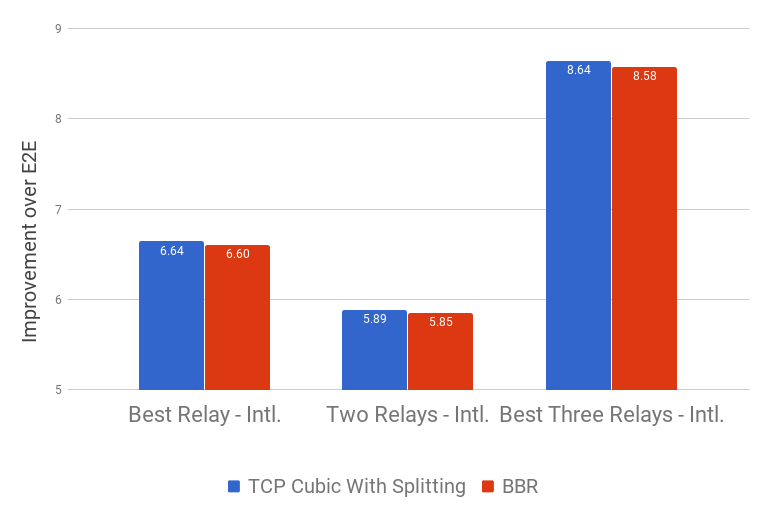
\includegraphics[width=0.47\textwidth]{figures/bbr.png}
%     \caption{TCP Cubic vs. BBR, using AWS relays}
%     \label{fig:tcp-vs-bbr}
% \end{figure}
%\AB{Do we want a CDF of BBR/TCP over all experiments?}


\subsection{Using Quick-Start TCP Pays Off}\label{subsec:quick-start}
%While the effects of congestion control in overlay networks have been discussed before(~\cite{CRONets}, \NR{are there any more?}), much is left unknown. We therefor conducted experiments on our relay machines in multiple scenarios, testing TCP without splitting, TCP Cubic with splitting, BBR~\cite{BBR} and aggressive TCP. \NR{@AB, can you fill our the details of the aggressive TCP?} 
\autoref{fig:aggressive} illustrates the impact of using Quick-Start TCP Cubic  instead of TCP Cubic or BBR.
%, in the same experimental settings as in \autoref{fig:tcp-vs-bbr}
We observe that (1) Quick-Start TCP significantly improves upon TCP Cubic and BBR, and (2) this improvement is particularly large with two or three relays. We hypothesize that their performance gain is similar because the main benefit of using the third (middle) relay is in reducing the impact of the slow-start phase by reducing the RTT, and Quick-Start TCP avoids slow-start altogether.

%\IK{here we need to explain what happens for (a) other clouds, (b) US. For instance, is it just a coincindence that perf(2 relays)=perf(3 relays)?}


% Next, we tested the performance of aggressive TCP.
% While the results varied from cloud provider to another, a trend did emerge: aggressive TCP yielded better, and in most cases using two or three relays, much better results than TCP Cubic (or BBR). In the experiment depicted in Figure~\ref{fig:aggressive} we used Azure nodes for relays.




%Th e effects of congestion control in overlay networks have received some attention in previous studies ( \NR{are there any more?}). We have decided to conduct a

\begin{figure}[!t]
  \centering
    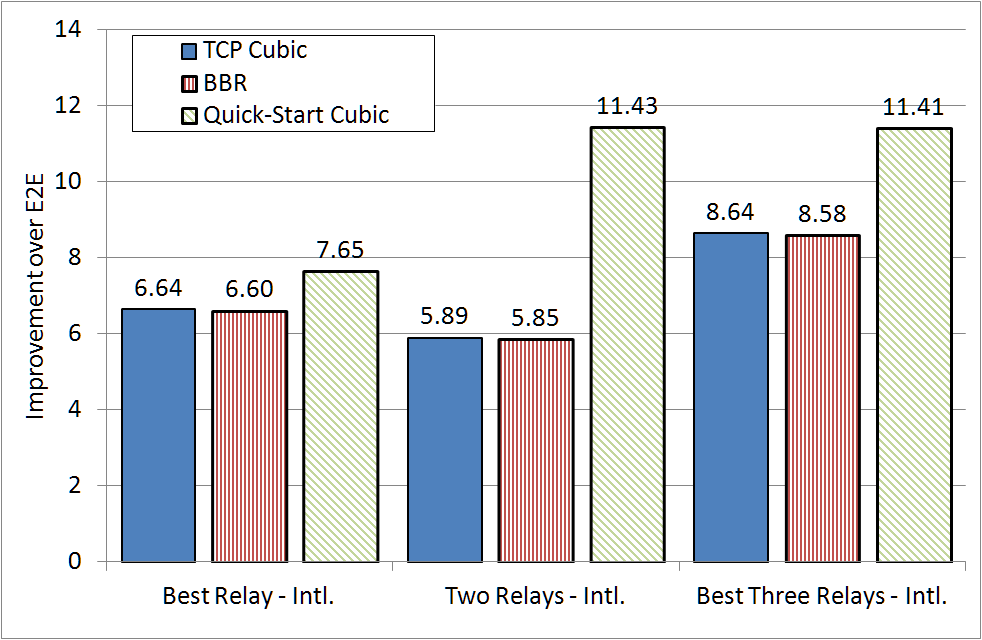
\includegraphics[width=0.47\textwidth,trim=2mm 2mm 2mm 2mm,clip]{figures/aggressive.png}
    \caption{Impact of Quick-Start TCP demonstrated using the Mumbai-SF international transmission of a large file with TCP splitting over AWS. In all three cases of best-single, simple-double and best-triple relays, Quick-Start TCP achieves remarkably higher efficiency. In the last two cases, it achieves an impressive 11.4$\times$ improvement over E2E.
   }
    \label{fig:aggressive}
\end{figure}



% \begin{figure}[t]
%   \centering
%     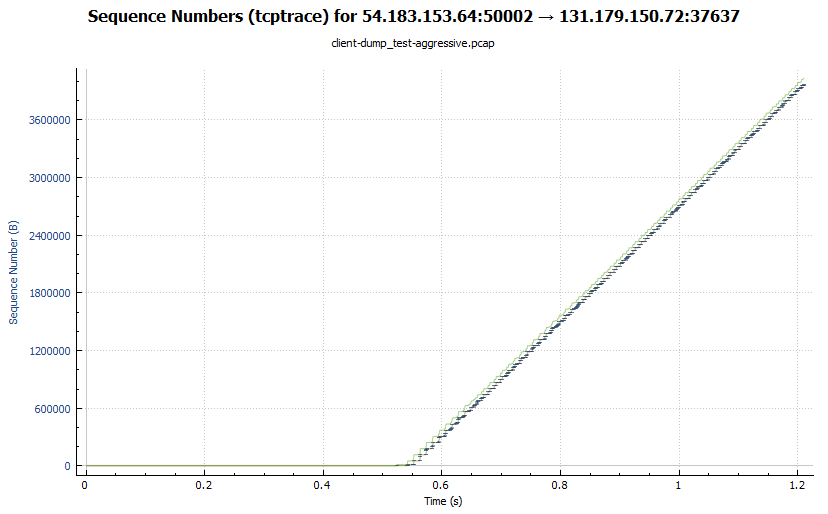
\includegraphics[width=0.47\textwidth]{figures/client-aggressive-tcptrace}
%     \caption{Client with limited rwin - with a close relay and aggressive TCP \AB{should this stay or go?}}
%     \label{fig:close-to-poor-client-benefit-aggressive}
% \end{figure}


\subsection{File Size Matters}
%\label{sec:file-sizes}
The previously-presented results are for large file downloads. What about small files? \autoref{fig:small-file} illustrates how our experimental results for small files exhibit similar trends in the international case: TCP splitting is better, and Quick-Start TCP helps. However, in the US case, in contrast to the large files, even the best results provide no improvement beyond simple E2E delivery. 

\begin{figure}[t]
  \centering
    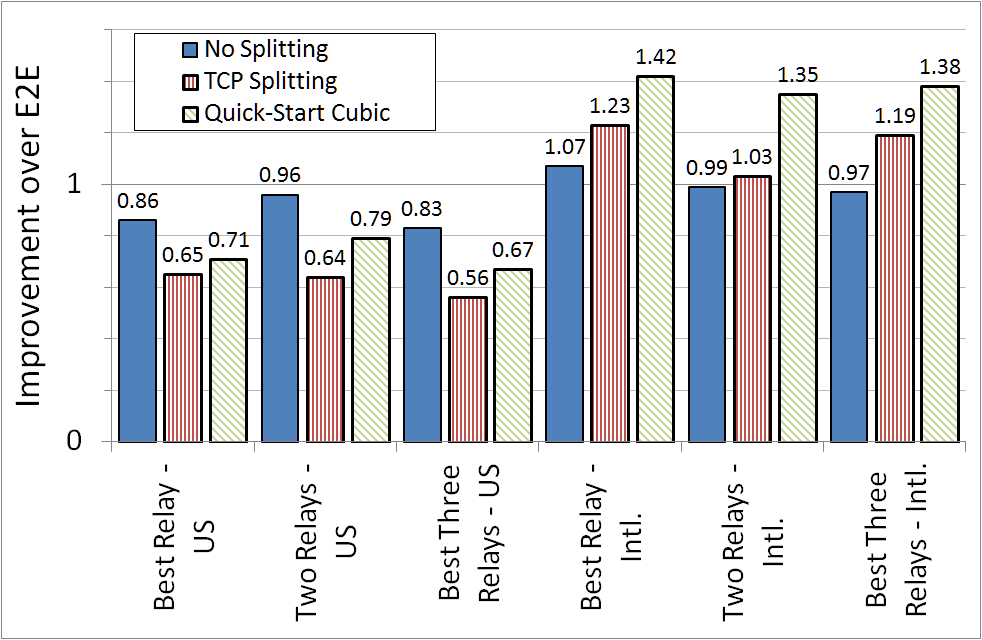
\includegraphics[width=0.47\textwidth,trim=2mm 2mm 2mm 2mm,clip]{figures/small_file}
    \caption{Small-file results using AWS relays. In the international Mumbai-SF case, TCP splitting performs better than non-splitting, and Quick-Start TCP further improves performance. However, in the US case, the best  results with splitting are still about 30\% lower than E2E.}
    \label{fig:small-file}
\end{figure}

\subsection{Is RTT a Good Proxy for Performance?}

In contrast to measuring bandwidth, measuring latency (in terms of RTT) is simple. When is RTT a good proxy for performance, in terms of download completion time?

\noindent{\bf Without TCP splitting.} When TCP is \emph{not} split, end-to-end RTT is a good proxy for download completion time: the shorter the RTT, the shorter the download. We used RTT measurements to estimate the improvement of different routing strategies over E2E by calculating the ratio between the E2E RTT and the RTT of the tested route. \autoref{fig:rtt-estimate-nat-1hop} plots the correlation between our estimator and the actual performance gain. % for single-relay (no TCP splitting).

\noindent{\bf With TCP splitting.} When TCP splitting is used, with Cubic as the congestion control algorithm, an RTT-measurements-based estimator succeeded in predicting the performance gain of the 3-relay method over the 2-relay method. This is accomplished by calculating the ratio of the RTT between \rc and \rs and the maximum RTT of the segments of the route through the third node used between them. Namely, if $\rtt(\rc,\rs)$ is the RTT between \rc and \rs, $\rtt(\rc,\rmid)$ is the RTT between \rc and the middle relay, and $\rtt(\rmid,\rs)$ is the RTT between \rs and the middle relay, we estimate that using this third relay would improve download time by 
\[
\frac{\rtt(\rc,\rs)}{\max(\rtt(\rc,\rmid),\rtt(\rmid,\rs))}
\]
compared to using the two-relay route using \rc and \rs only.
The reasoning behind this estimator is that when splitting is used, the throughput is limited by the slowest segment of the route. \autoref{fig:rtt-estimate-ssh-3hop} depicts the correlation between this estimator and the actual gain of the 3-relay method over the 2-relay method (both with TCP splitting at each relay).

Motivated by the relative accuracy of this estimator, we used RTT measurements to predict which 4-relay route would fare best when using TCP splitting and Cubic as the congestion control protocol. The 4-relay route achieved an improvement of 8.57$\times$, \ie higher than the 7.38$\times$ improvement achieved with the 3-relay route calculated with min-max RTT between \rc and \rs. 
%In \autoref{fig:4-relay-route-cubic} we compare the route found using this method to the best 3-relay route and the 2-relay method. 
 
We point out that, in contrast to the above results, this estimator fails to provide good results for the single relay with TCP splitting strategy, possibly because as RTTs get higher the impact of congestion and loss rate becomes more significant.
%\AB{Do we want a section about using RTT as an estimator of TCP performance?} \IK{please give us a plot draft so we can decide what we have to answer; this can join the lesson (1) of Figure 2, or the part of Figure 3.}


\begin{figure}[t]
  \centering
  
    \begin{subfigure}{0.47\columnwidth}
  \centering
  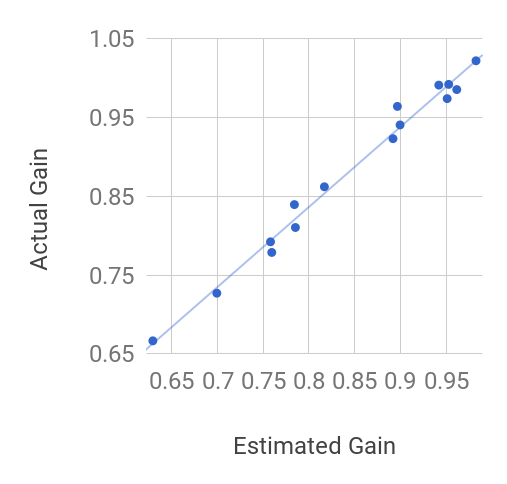
\includegraphics[width=\columnwidth]{figures/gainEstimateVsActual-nat-1hop-newer}
    \caption{}
    \label{fig:rtt-estimate-nat-1hop}
\end{subfigure} \hfill
\begin{subfigure}{0.47\columnwidth}
  \centering
  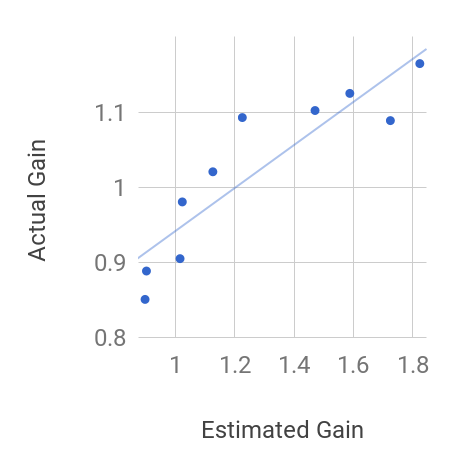
\includegraphics[width=\columnwidth]{figures/gainEstimateVsActual-ssh-3hop-newer}
    \caption{} \label{fig:rtt-estimate-ssh-3hop}
\end{subfigure}
    \caption{Performance gain estimates \vs actual gain of \textbf{(a)} the single relay method without splitting; and \textbf{(b)} the 3 relay setup with splitting.}
\end{figure}

%\begin{figure}
%  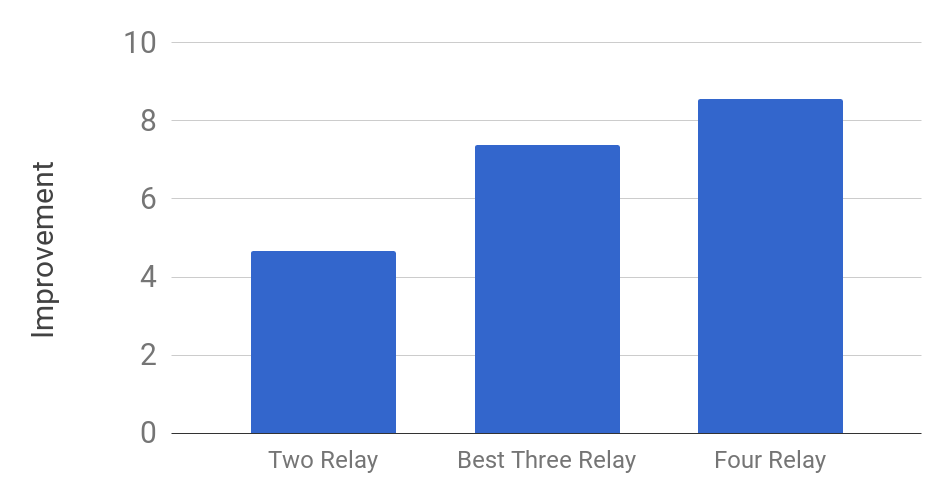
\includegraphics[width=0.47\textwidth]{figures/4relaysVs2and3}
%    \caption{Results of a 4-relay route with TCP splitting using TCP cubic. 4-relay route chosen as min-max route between \rc and \rs using RTT measurements. The graph depicts improvement over the E2E method when using SF as client, Mumbai as server and using cloud nodes on Azure. The nodes used in the 4-relay route are westus$\to$japaneast$\to$southeastasia$\to$westindia.}
%    \label{fig:4-relay-route-cubic}
%\end{figure}



% In case we do have room for the graph:
% This is exemplified by the sequence number graphs we present in \autoref{fig:close-to-poor-client-benefit}

% \begin{figure}[t]
%   \centering
%     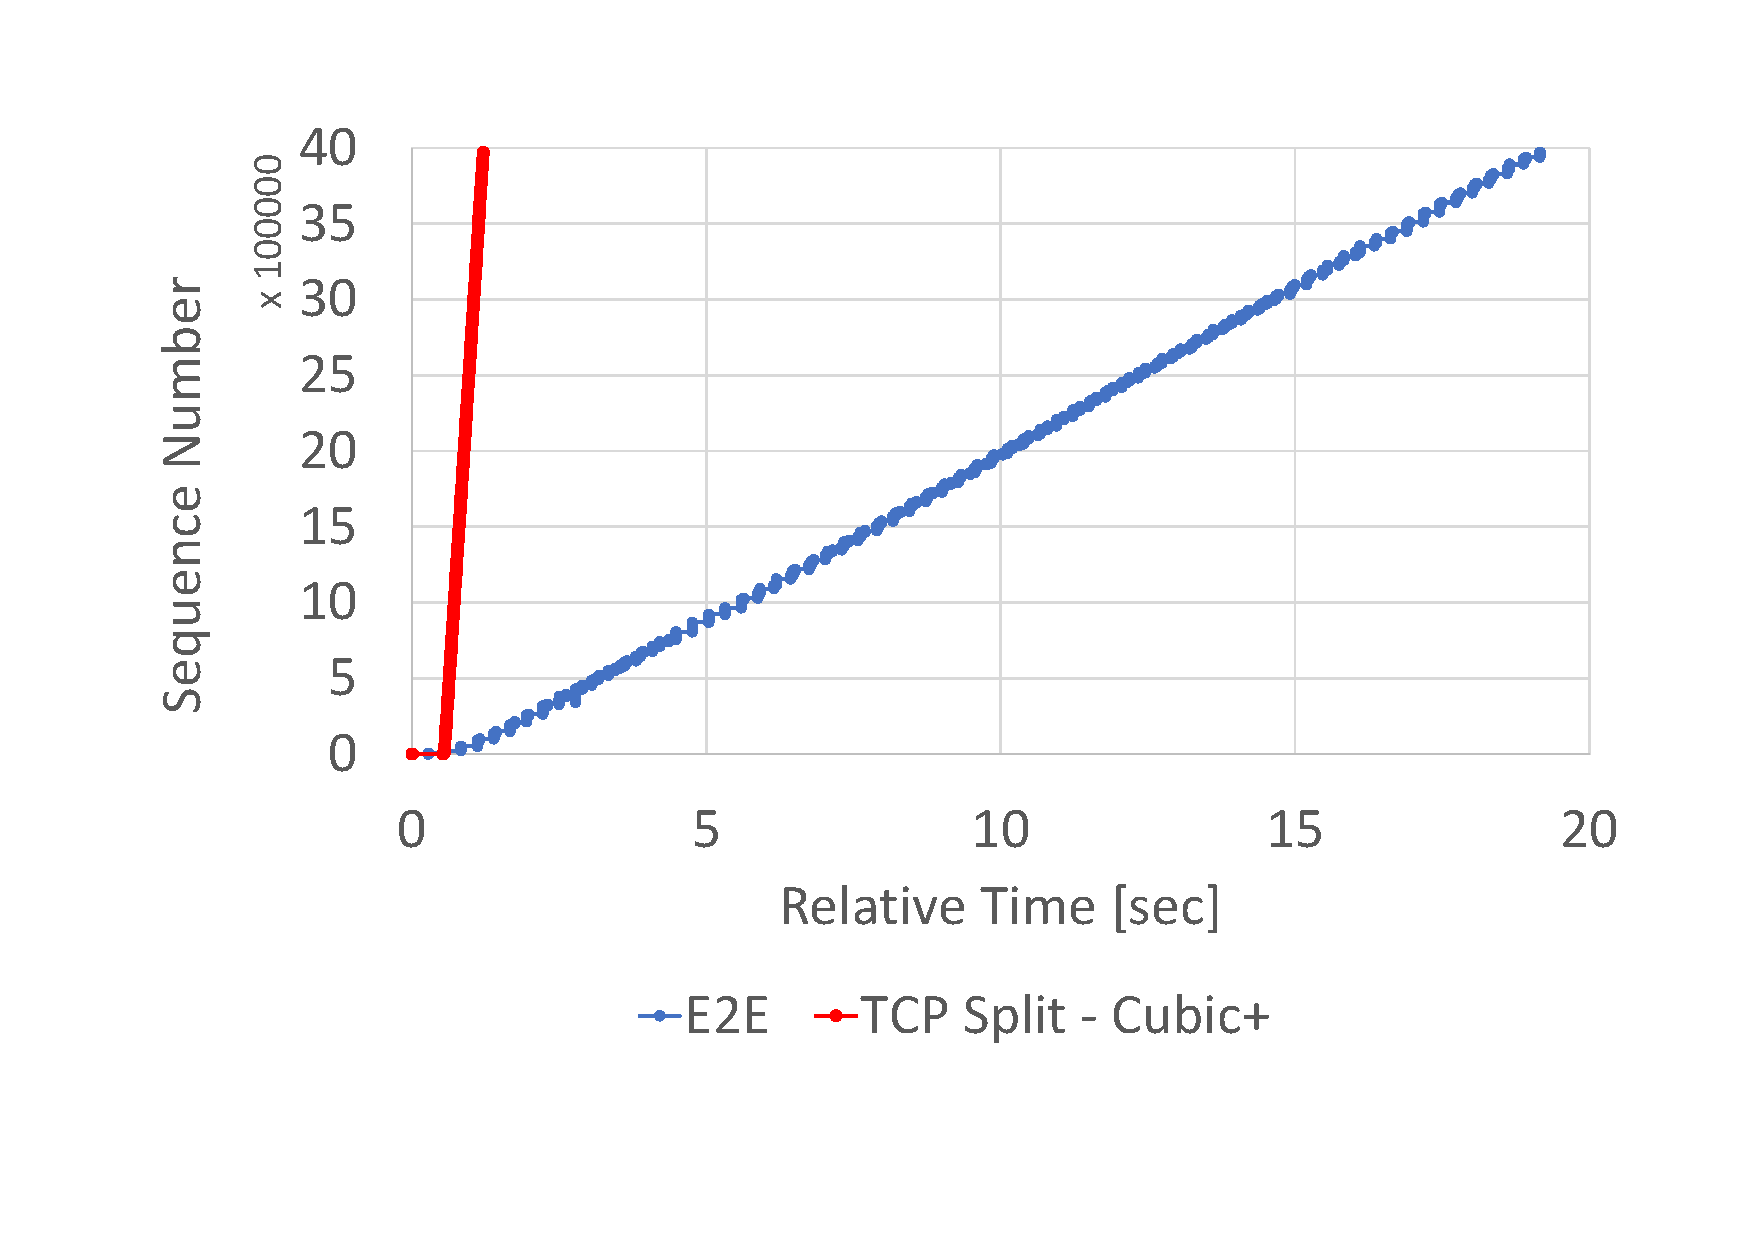
\includegraphics[width=0.47\textwidth]{figures/client-e2eVsAggressive}
%     \caption{Client with limited rwin. The receive window and the RTT set the throughput. This graph compares the sequence number of the first byte in each received packet between the E2E method and the 2-relay TCP split using Quick Start Cubic}
%     \label{fig:close-to-poor-client-benefit}
% \end{figure}


% \section{Related Work}

% \EZ{\cite{le2016understanding} is a 5 pages workshop (CAN'16) from IBM's group (CRONets). 
% They make very strong claims: (1) the bottleneck is not the overlay but the Internet path to get to the cloud (2) simple forwarding (without a proxy/split) gains only 13\% (3) "multi-hop indirection" (their terminology) do not add to single-hop.
% Comparison to us: (1) worked with one cloud only (IBM) (2) their single server is inside their cloud (3) never really checked multi-hop (4) the clients are located in IBM's branches which is not exactly "outside the overlay" (5) do not mention congestion control even once.}

% \T{Internet overlays.} The idea of overlay networking on top of the Internet dates back almost two decades~\cite{old-overlay-1, old-overlay-2, RON}. Many studies established that the default BGP path between two end-points is often inferior to an alternate path traversing an overlay network~\cite{old-overlay-1, old-overlay-2, RON, akamai-2, akamai-3, akamai-4}. Akamai's SureRoute service relies on such an Internet overlay network.

% \T{Cloud overlays.} Recently, overlay networking through the \emph{cloud} has received attention from both researchers (e.g.,~\cite{CRONets}) and practitioners (e.g.,~\cite{teridion}). CRONets~\cite{CRONets} leverages a \emph{single} cloud relay with TCP splitting for data delivery. Our experimentation with a broad spectrum of routing and congestion control schemes for cloudified data delivery, suggests that cloud overlays can provide significantly higher performance than that achievable using only a single relay.
% % \EZ{I think we can stop here. Why would we like to present more of their findings?} and show that up to 50\% of the paths do not improve their throughput by going to the cloud when TCP splitting is disabled. 
% %provides a strong argument in favor of this transit point. However, unlike in the \name overlay network that relies on a full routing solution through the cloud, CRONets only relies on a single-hop transit through the cloud. 
% %However, they neither consider more than one cloud relay, nor accelerated solutions like our quick-start TCP. \IK{How can we make this stronger?}
% %\EZ{Instead, we can use their own future-work statement. Something like this} 

% \T{Cloud-based content delivery.} The use of an HTTP proxy~\cite{cgn2017} in static AWS locations was shown to reduce webpage load times by half, when accessing remote websites. Cloud-based mobile browsing~\cite{zhao2011reducing,wang2013accelerating} is a common technique for reducing cellular costs and decreasing download times.

% \T{Cloud connectivity and performance.} \cite{one-hop} shows that some 60\% of end-user prefixes are within one-AS-hop from GCP (Google Cloud Platform). A different study~\cite{cgn2017} established that AWS has at least one node within a median RTT of merely 4.8~ms from servers hosting the top 10k most popular Web sites. \cite{unusual} shows that modern clouds have unusual internal routing structures that are hard to infer and CLAudit \cite{multidimensional} points out the increasing reliability of cloud latency. 

% \T{TCP Split.} Several papers considered TCP split to better TCP performance, \eg overcome different link characteristics~ \cite{Kopparty2002} (wired and wireless), compensate for very long RTTs in satellite links \cite{luglio2004}, and reduce search query latency~\cite{pathak2010measuring}. 
% Pucha and Hu explore TCP overlay \cite{pucha2005overlay, pucha2005slot}. 

% % Teridion~\cite{teridion} has recently announced it is using cloud overlay networks as an alternative to support the acceleration of dynamic content in the context of CDN networks. %\IK{Can we weaken this first sentence? If not, how strong is our novelty?} \IC{I don't think companies that do not disclose how they solve these problems are a big  
% % %dynamic content in the context of CDN networks. 
% % % Teridion seems to implement an overlay network over the public cloud that optimizes routes and TCP performance to carry a CDN-like acceleration for dynamic web and SaaS services. 
% % The Teridion network accelerates the downloads and Web interaction for service providers (\eg Box, Egnyte) for dynamic transactions or private content that traditional CDN technology cannot support. Therefore, unlike CLEAN, % that provides full corporate connectivity over a business-type Internet, 
% % the Teridion network does not provide connectivity between branch offices, datacenters and mobile users, has a single destination per customer, and does not provide any secure VPN connections or any reliability guarantees.  Unfortunately, they have also not disclosed the details of their internal architecture. 

% % Incidentally, Akamai~\cite{akamai} has also introduced a new service termed ``Dynamic Site Acceleration" that is based on TCP split and optimal routing between Akamai edge servers. However, they are not using the public clouds.  





% %\T{Resilient overlay networks}. The Resilient Overlay Network (RON)~\cite{RON} establishes an overlay network that can quickly restore communication following failures that disconnect Internet paths. The authors argue that in practical Internet environments, RON only takes tens of seconds for the routing algorithms to detect and reroute around failures. RON is implemented in several locations on top of private servers. It uses distributed link-state routing algorithms between these servers. Since RON is an early work (2001), it does not take advantage of the public cloud compute and high-speed networking infrastructure and guarantees as well as of SDN-based architectures. As the main goal of RON is to circumvent Internet failures, it also does not split TCP connections or deal with QoS and security issues related with a global business Internet.

% %\T{Leased backbone.} Additional companies address the relocation of corporate WANs to a network service through the introduction of a specialized backbone network rather than using the public clouds, \eg Aryaka~\cite{aryaka}, Cato Networks~\cite{cato} and Virtela~\cite{virtela}. 

% %\T{SD-WAN.} A large number of companies is solving the problem of backhauled Internet traffic over expensive corporate WANs by downloading and uploading Internet traffic from the branch office directly to the Internet, without passing through the corporate secure gateway. Since corporations insist that this traffic must be secured and inspected, the firewall and other security functions are distributed to the branch offices and managed centrally. Our \name network can help provide a better and more reliable performance to this Internet-based traffic.

% %\T{Cloud destination.} FootPrint~\cite{footprint} provides an integrated system for jointly allocating the right cloud proxy and datacenter to each client as well as routing through the best route. Its goal is to access a cloud datacenter destination by using the WAN, while the goal of \name is to build an overlay on the cloud to replace the corporate WAN and therefore to exploit the cloud inter-connection network, even when accessing a SaaS website.

% % \T{Full network path.} ARROW~\cite{arrow} allows users to configure reliable
% % and secure end-to-end paths through a set of different providers. 
% % %In contrast, by controlling all links within its network, \name enables a uniform security guarantee that can easily be strengthened.
% % In addition, \cite{nira} suggests a new Internet routing architecture (NIRA) that gives a user the ability to choose the sequence of providers his packets take. The goal of \name, in contrast, is to obtain a single cloud overlay provider.

\section{Fairness}

We were wondering whether Quick-Start Cubic is too aggressive and unfair towards other regular TCP flows. By essentially skipping the slow-start phase of TCP, even though we keep the connection remainder unchanged, aren't we just hogging the link and exploiting a loophole
that cloud providers should soon close?
\autoref{fig:agg-vs-cubic} looks at the per-byte download time of our large file in the cloud. We learn that (1) the average throughput is clearly higher for the Quick-Start TCP, as expected from \autoref{fig:aggressive}; but (2) this is mainly because TCP cubic tends to operate in a sporadic bursty manner in its slow-start, by first waiting for a full RTT for a bunch of ACKs to arrive back to the server, then sending bursts of packets to catch up. When zooming on the TCP-cubic bursts, its slope surprised us by being higher than for the Quick-Start TCP, \ie it is \textit{more} aggressive because of this catching up. 
\begin{figure}[!t]
  \centering
    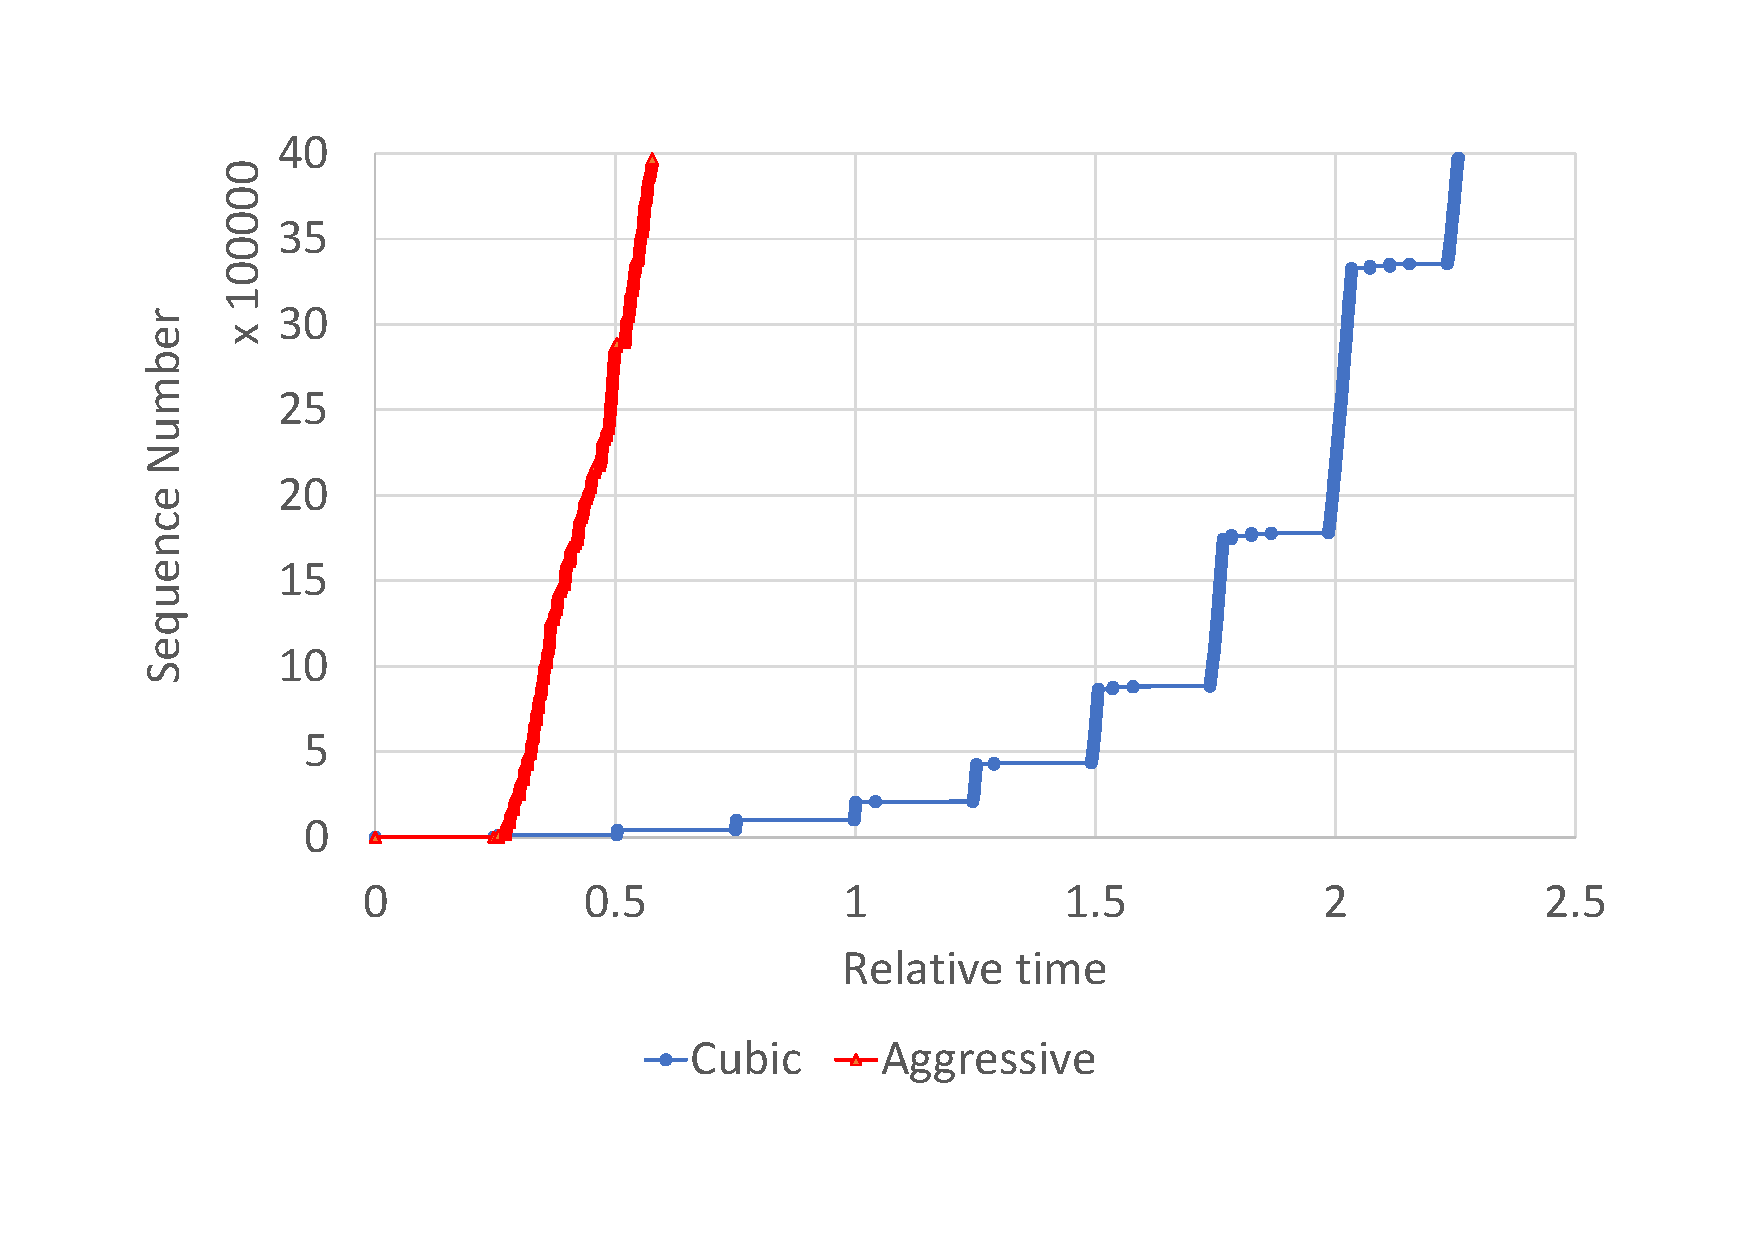
\includegraphics[width=0.47\textwidth,trim=2mm 2mm 2mm 2mm,clip]{figures/CubicVsAggressive-seq}
    \caption{Per-byte look at the flow between \rs and \rc, as captured on \rc. The graphs depict the sequence number received \vs relative time (to the beginning of the TCP connection). The transmission rate during the bursts in the default cubic option is 260 MBps while it is only 110 Mbps when the Quick-Start option is used. However, since Quick-Start avoids slow-start, its overall download time is much shorter.  
    %Why aggression pays off
    }
    \label{fig:agg-vs-cubic}
\end{figure}

\section{Related Work}
\EZ{ \cite{le2016understanding} is a 5 pages workshop (CAN'16) from IBM's group (CRONets). They make very strong claims: (1) the bottleneck is not the overlay but the Internet path to get to the cloud (2) simple forwarding (without a proxy/split) gains only 13\% (3) "multi-hop indirection" (their terminology) do not add to single-hop. Comparison to us: (1) worked with one cloud only (IBM) (2) their single server is inside their cloud (3) never really checked multi-hop (4) the clients are located in IBM's branches which is not exactly "outside the overlay" (5) do not mention congestion control even once.}

\EZ{ \cite{siracusano2016miniproxy} claim that since a proxy has proven to be beneficial, and it is important to put it in the middle of a connection, then there is a need for lightweight proxy that can be installed anywhere is a very short time. They implemented a novel TCP proxy that (1) boots quickly in 12ms (2) has a very small memory footprint of 6MB (3) uses early SYN forwarding with \texttt{tcp\_early\_syn\_bind()} (4) built over \texttt{unikernels}.}

% Mohammad Alizadeh
\EZ{ \cite{jeyakumar2012eyeq} partially support our claim that the cloud's network can be treated as a limitless network resource.}

% Mohammad Alizadeh
\EZ{ \cite{narayan2017ccp} offers to move congestion control off the datapath and into a separate, reusable,
and flexible user-space agent called CCP. Although this is basically a discussion paper (Hotnets...), the background seems relevant to ours, mainly because they mention the growing need for new solutions - high-speed, existing bypasses, QUIC, etc. }

% Mohammad Alizadeh and Aditya Akella
\EZ{ Several ideas were presented over the years to adapt congestion control mechanisms to modern data centers and/or clouds. Among them are DCTCP~\cite{alizadeh2010dctcp} that was specific to fast datacenters, and the later AC/DC~\cite{keqiang2016acdc} that aims to allow a cloud provider to utilize DCTCP (and similar), without having control over the VM or requiring changes in network hardware, by implementing congestion control in the vSwitch running on each server.}

% Hitesh Ballani
\EZ{Past studies of cloud providers have found that both the bandwidth and packet delay across their network can vary by an order of magnitude. More recent papers, such as \cite{jang2015silo}, offer a mechanism for predictable network performance in the cloud, supporting out own findings during this study.}

% Sachin Katti
\EZ{\cite{chakravorty2003aggregation} puts a transparent proxy in GPRS networks to split TCP connections into two halves, the wired and wireless sides. They emphasize that GPRS, like other wide-area wireless networks, exhibits many bad characteristics in terms of TCP and HTTP performance, leading to a need to separate that link from the more reliable path from the wireless gateway to the other end. The study of these characteristics in real networks, also justifies the location of the proxy, something we can also mention in our paper.}

% Mohammad Alizadeh and Sachin Katti
\EZ{\cite{jose2015proactive} advocates proactive congestion control mechanisms that explicitly calculate sending rates based on flow.}

\EZ{\cite{le2015experiences} presents IBM's experience with a transparent TCP proxy sitting close to wireless clients. One of their relevant findings is that the success of the deployment highly depends on the location of the proxy.}

\EZ{Google's work~\cite{flach2013reducing} reduce download completion times by adding judicious redundancy to TCP. They offer 3 easily-deployable mechanisms (active, reactive, and corrective), and show experimental results that decrease both mean time and 99th percentile latency in Google's traffic.}

% Amin Vahdat - many relevant papers
\EZ{We can mention TIMELY~\cite{mittal2015timely} that adjusts transmission rates using RTT gradients to keep packet latency low while delivering high bandwidth. They implement their idea in software running over NICs with OS-bypass capabilities.
}

% Olivier Bonaventure - many MPTCP papers
\EZ{Do you think MPTCP~\cite{barre2010mptcp} is relevant? MPTCP requires a modification of both ends, making it hard to deploy and use in practice. This alone makes a good case for having two relays fully controls by us.}

\T{Internet overlays.} The idea of overlay networking on top of the Internet dates back almost two decades~\cite{old-overlay-1, old-overlay-2, RON}. Many studies established that the default BGP path between two end-points is often inferior to an alternate path traversing an overlay network~\cite{old-overlay-1, old-overlay-2, RON, akamai-2, akamai-3, akamai-4}. Akamai's SureRoute service relies on such an Internet overlay network.

\T{Cloud overlays.} Recently, overlay networking through the \emph{cloud} has received attention from both researchers (e.g.,~\cite{CRONets}) and practitioners (e.g.,~\cite{teridion}). CRONets~\cite{CRONets} leverages a \emph{single} cloud relay with TCP splitting for data delivery. Our experimentation with a broad spectrum of routing and congestion control schemes for cloudified data delivery, suggests that cloud overlays can provide significantly higher performance than that achievable using only a single relay.
% \EZ{I think we can stop here. Why would we like to present more of their findings?} and show that up to 50\% of the paths do not improve their throughput by going to the cloud when TCP splitting is disabled. 
%provides a strong argument in favor of this transit point. However, unlike in the \name overlay network that relies on a full routing solution through the cloud, CRONets only relies on a single-hop transit through the cloud. 
%However, they neither consider more than one cloud relay, nor accelerated solutions like our quick-start TCP. \IK{How can we make this stronger?}
%\EZ{Instead, we can use their own future-work statement. Something like this} 

\T{Cloud-based content delivery.} The use of an HTTP proxy~\cite{cgn2017} in static AWS locations was shown to reduce webpage load times by half, when accessing remote websites. Cloud-based mobile browsing~\cite{zhao2011reducing,wang2013accelerating} is a common technique for reducing cellular costs and decreasing download times.

\T{Cloud connectivity and performance.} \cite{one-hop} shows that some 60\% of end-user prefixes are within one-AS-hop from GCP (Google Cloud Platform). A different study~\cite{cgn2017} established that AWS has at least one node within a median RTT of merely 4.8~ms from servers hosting the top 10k most popular Web sites. \cite{unusual} shows that modern clouds have unusual internal routing structures that are hard to infer and CLAudit \cite{multidimensional} points out the increasing reliability of cloud latency. 

\T{TCP Split.} Several papers considered TCP split to better TCP performance, \eg overcome different link characteristics~ \cite{Kopparty2002} (wired and wireless), compensate for very long RTTs in satellite links \cite{luglio2004}, and reduce search query latency~\cite{pathak2010measuring}. 
Pucha and Hu explore TCP overlay \cite{pucha2005overlay, pucha2005slot}. 

% Teridion~\cite{teridion} has recently announced it is using cloud overlay networks as an alternative to support the acceleration of dynamic content in the context of CDN networks. %\IK{Can we weaken this first sentence? If not, how strong is our novelty?} \IC{I don't think companies that do not disclose how they solve these problems are a big  
% %dynamic content in the context of CDN networks. 
% % Teridion seems to implement an overlay network over the public cloud that optimizes routes and TCP performance to carry a CDN-like acceleration for dynamic web and SaaS services. 
% The Teridion network accelerates the downloads and Web interaction for service providers (\eg Box, Egnyte) for dynamic transactions or private content that traditional CDN technology cannot support. Therefore, unlike CLEAN, % that provides full corporate connectivity over a business-type Internet, 
% the Teridion network does not provide connectivity between branch offices, datacenters and mobile users, has a single destination per customer, and does not provide any secure VPN connections or any reliability guarantees.  Unfortunately, they have also not disclosed the details of their internal architecture. 

% Incidentally, Akamai~\cite{akamai} has also introduced a new service termed ``Dynamic Site Acceleration" that is based on TCP split and optimal routing between Akamai edge servers. However, they are not using the public clouds.  





%\T{Resilient overlay networks}. The Resilient Overlay Network (RON)~\cite{RON} establishes an overlay network that can quickly restore communication following failures that disconnect Internet paths. The authors argue that in practical Internet environments, RON only takes tens of seconds for the routing algorithms to detect and reroute around failures. RON is implemented in several locations on top of private servers. It uses distributed link-state routing algorithms between these servers. Since RON is an early work (2001), it does not take advantage of the public cloud compute and high-speed networking infrastructure and guarantees as well as of SDN-based architectures. As the main goal of RON is to circumvent Internet failures, it also does not split TCP connections or deal with QoS and security issues related with a global business Internet.

%\T{Leased backbone.} Additional companies address the relocation of corporate WANs to a network service through the introduction of a specialized backbone network rather than using the public clouds, \eg Aryaka~\cite{aryaka}, Cato Networks~\cite{cato} and Virtela~\cite{virtela}. 

%\T{SD-WAN.} A large number of companies is solving the problem of backhauled Internet traffic over expensive corporate WANs by downloading and uploading Internet traffic from the branch office directly to the Internet, without passing through the corporate secure gateway. Since corporations insist that this traffic must be secured and inspected, the firewall and other security functions are distributed to the branch offices and managed centrally. Our \name network can help provide a better and more reliable performance to this Internet-based traffic.

%\T{Cloud destination.} FootPrint~\cite{footprint} provides an integrated system for jointly allocating the right cloud proxy and datacenter to each client as well as routing through the best route. Its goal is to access a cloud datacenter destination by using the WAN, while the goal of \name is to build an overlay on the cloud to replace the corporate WAN and therefore to exploit the cloud inter-connection network, even when accessing a SaaS website.

% \T{Full network path.} ARROW~\cite{arrow} allows users to configure reliable
% and secure end-to-end paths through a set of different providers. 
% %In contrast, by controlling all links within its network, \name enables a uniform security guarantee that can easily be strengthened.
% In addition, \cite{nira} suggests a new Internet routing architecture (NIRA) that gives a user the ability to choose the sequence of providers his packets take. The goal of \name, in contrast, is to obtain a single cloud overlay provider.


\section{Conclusion}
We initiated the systematic exploration of cloudified data delivery and presented initial results suggesting that optimization of performance should be viewed through the congestion-control lens.  We view cloudified data delivery as a promising direction for overcoming the inefficiencies of today's routing (BGP) and congestion control (TCP) protocols. We thus argue that tapping the full potential of this approach is of great importance. 

Our results leave many important questions wide open. We discuss some of these below.

\T{Cloudified data delivery vs. state-of-the-art end-to-end congestion control.} Recent studies claim to improve performance by an order of magnitude by employing better congestion control protocols end-to-end~\cite{PCC}. How does this compare to cloudified data delivery? Could routing through the cloud be redundant?

\T{Modeling the cloud.} Though we provided intuitions for our empirical results, the root causes underlying our results remain hidden. We believe that more thought should be given to generating (from empirical observations) models of the cloud(s) that can provide insights into its inner workings.

\T{Is Quick-Start TCP too aggressive?} Our results (\S\ref{subsec:quick-start}) provide partial evidence that Quick-Start TCP is not necessarily more aggressive to other connections than regular TCP. Providing better empirical support of this claim is crucial, as better performance for cloud users should not (arguably) come at the cost of harming others.

\AB{A couple of general comments / points:
The biggest benefits to OCD we see are due to limited send window in the sender or limited rwin in the receiver. These limitation are due to one of the following:
\begin{itemize}
    \item  A web server that is loaded might manage its memory resource in a way that would limit the socket tx buffer for its TCP connections, thus limiting the maximum allowed send window. This limits the send rate for remote clients with higher RTTs.
    \item A ``weaker'' client, with limited memory resources would limit the rwin it can report to the sender, again limiting the throughput to $\frac{\mbox{rwin}}{\mbox{RTT}}$. This is probably a typical case for IoT devices.
    \item In the other direction, a client with limited memory would have lower throughput when sending traffic over the Internet to a remote server, since it has limited memory for the socket buffer. 
\end{itemize}
caveat to the last two bullets - the statements are true for IoT devices connecting directly to servers over the Internet. However, I think there is an IoT gateway that's supposed to aggregate information from IoT devices in its vicinity, and in that case there are no long-haul TCP connections ending in, or originating at the IoT device itself.}



\begin{comment}

\section*{Acknowledgments}
Chen, Shay, Sujata

\end{comment}

\appendix

% \bibliographystyle{abbrv}
\bibliographystyle{acm}
% \begin{small}
\bibliography{mybib,overlaybib,sigcomm18}
% \bibliography{sigcomm18}
% \end{small}

%\bibliographystyle{plain}
%%\bibliography{abb,ultimate}

%\newpages

\end{document}